\documentclass[aspectratio=169,11pt]{beamer}

% Shared style (ib-tutorials.sty at the repo root).
\makeatletter\def\input@path{{./}{../}}\makeatother
\usepackage{ib-tutorials}

\usepackage[utf8]{inputenc}
\usepackage{amsmath,amssymb}
\usepackage{booktabs}
\usepackage{array}
\newcolumntype{L}[1]{>{\raggedright\arraybackslash}p{#1}}
\usepackage{graphicx}
\graphicspath{{../pictures/5-visit/}{pictures/5-visit/}}
\usepackage{xcolor}
\usepackage{listings}
\usepackage{tikz}
\usetikzlibrary{arrows.meta,positioning,shapes.geometric,fit,calc}
\usepackage{hyperref}

\newcommand{\sourcecredit}[1]{\vfill\begin{flushright}\tiny\textcolor{DarkGray}{#1}\end{flushright}}
\newcommand{\gui}[1]{\textsf{\textbf{#1}}}

\lstset{
  basicstyle=\ttfamily\scriptsize\color{BlackGray},
  keywordstyle=\color{NavyBlue}\bfseries,
  commentstyle=\color{DarkGray}\itshape,
  stringstyle=\color{OliveGreen},
  showstringspaces=false,
  columns=fullflexible,
  keepspaces=true,
  breaklines=true,
  breakindent=1em,
  frame=single,
  framerule=0.4pt,
  rulecolor=\color{LightGray},
  backgroundcolor=\color{LightGray!30},
  xleftmargin=0.25em,
  xrightmargin=0.25em
}
\lstdefinestyle{shell}{morecomment=[l]{\#}}
\lstdefinestyle{input}{morecomment=[l]{//}}
\lstdefinestyle{python}{morecomment=[l]{\#}}
\lstdefinestyle{data}{}
\lstdefinestyle{tiny}{basicstyle=\ttfamily\tiny\color{BlackGray}}
\lstdefinestyle{inputtiny}{morecomment=[l]{//},basicstyle=\ttfamily\tiny\color{BlackGray}}

\title[VisIt: getting started]{VisIt: getting started, and making it look better}
\subtitle{Opening an IBAMR run in VisIt: the points, the fields, the time slider; the plot attributes that turn the first picture into a figure; annotations, sessions, saving pictures; the same steps for IB2d}
\author[Miller]{Laura A. Miller}
\institute[UArizona]{Department of Mathematics, University of Arizona}
\date{Using IB Software \textbullet\ Part V \textbullet\ Chapter 26}

\begin{document}

% 1
\begin{frame}[plain]
\maketutorialtitlepanel{%
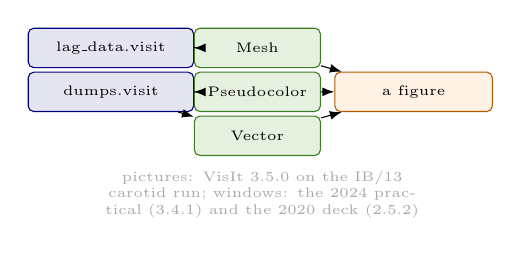
\begin{tikzpicture}[scale=0.62, every node/.style={font=\tiny}]
  \node[draw=NavyBlue,fill=NavyBlue!10,rounded corners=2pt,minimum width=2.1cm,minimum height=0.5cm] (a) at (0,0) {\code{lag\_data.visit}};
  \node[draw=NavyBlue,fill=NavyBlue!10,rounded corners=2pt,minimum width=2.1cm,minimum height=0.5cm] (b) at (0,-0.9) {\code{dumps.visit}};
  \node[draw=OliveGreen,fill=OliveGreen!10,rounded corners=2pt,minimum width=1.6cm,minimum height=0.5cm] (m) at (3,0) {Mesh};
  \node[draw=OliveGreen,fill=OliveGreen!10,rounded corners=2pt,minimum width=1.6cm,minimum height=0.5cm] (p) at (3,-0.9) {Pseudocolor};
  \node[draw=OliveGreen,fill=OliveGreen!10,rounded corners=2pt,minimum width=1.6cm,minimum height=0.5cm] (v) at (3,-1.8) {Vector};
  \node[draw=orange!70!black,fill=orange!10,rounded corners=2pt,minimum width=2.0cm,minimum height=0.5cm] (f) at (6.2,-0.9) {a figure};
  \draw[-{Latex[length=1.5mm]}] (a) -- (m); \draw[-{Latex[length=1.5mm]}] (b) -- (p); \draw[-{Latex[length=1.5mm]}] (b) -- (v);
  \draw[-{Latex[length=1.5mm]}] (m) -- (f); \draw[-{Latex[length=1.5mm]}] (p) -- (f); \draw[-{Latex[length=1.5mm]}] (v) -- (f);
  \node[text=DarkGray,align=center,text width=5.4cm] at (3.1,-3.0) {pictures: VisIt 3.5.0 on the IB/13 carotid run; windows: the 2024 practical (3.4.1) and the 2020 deck (2.5.2)};
\end{tikzpicture}}
\end{frame}

% 2
\begin{frame}{Learning goals}
\label{fr:goals}
\footnotesize By the end of this chapter you should be able to:
\begin{enumerate}
  \item install the current VisIt and open the two files an IBAMR run writes for it, the Lagrangian points and the fluid dumps, as two sources in one window;
  \item draw the boundary as a Mesh plot and the fields as Pseudocolor and Vector plots, step through time with both sources in step, zoom, and reset the view;
  \item use the plot attribute windows for the things that matter: fixed limits, nodal centering, opacity, the colour table, the number, scale and colour of vectors, the size and width of the boundary;
  \item turn off what a figure does not need (database name, user name, grid lines, legends you did not ask for), label the axes, place a legend, add a text box;
  \item save a picture at a chosen resolution, save and restore a session, and know where movies are made (chapter 30);
  \item do the same with IB2d's \code{.vtk} files, and apply the five rules of a readable figure from the 2015 graph supplement.
\end{enumerate}
\begin{punchbox}
\scriptsize The pictures of plots are new, rendered with VisIt 3.5.0 from a run you can make yourself in three and a half minutes (IB/13, the human carotid). The window screenshots are the 2024 practical's (VisIt 3.4.1, the same windows as 3.5) and, where that deck has none, the 2020 deck's (VisIt 2.5.2); the text names the 3.x controls. A re-shoot in 3.5 is planned (\code{plan/visit-screenshots-todo.md}).
\end{punchbox}
\end{frame}

% 3
\begin{frame}{Where this chapter comes from}
\label{fr:sources}
\scriptsize
\begin{itemize}
  \item \al{``VISIT -- How to visualize IBAMR Data'' (2020, 31 slides; \code{DataViz\_Lecture\_1}):} the walk-through this chapter follows: download, preferences, open \code{lag\_data.visit}, add the mesh, draw, open \code{dumps.visit}, hide the coloured boxes, Pseudocolor of the vorticity, customize (limits $\pm5$, nodal, opacity 70\%), play, Vector U (uniform, $\sim$8000 vectors, constant colour), zoom, Save movie (MPEG), then the ``suggestions'' slides: hide the grid, 25\% of the original limits, nodal, vertices with a larger pixel size, legend off, database and user information off, axes titles and fonts, legend position, text boxes, sessions, movies as PNG frames joined in VirtualDub or QuickTime Pro. Its 21 screenshots are VisIt 2.5.2 on a Mac; nine are reused here.
  \item \al{The IB2d practical (2024, VisIt 3.4.1; slides 11--27):} the same walk-through for IB2d's \code{.vtk} databases (\code{lagsPts}, \code{u}, \code{omega}, \code{p}), the ``Index'' database correlation prompt, Hide/Show, the time arrows and the reset-view camera; the only VisIt 3.x screenshots in the collection, eleven of them reused here.
  \item \al{The 2013--2019 ``How to make it look better'' decks and the 2015 and 2019 course lectures:} tips folded in: the AMR levels as a Subset plot, ``Vector plot yielded no data at $t = 0$'', vertices as spheres, supersaturated limits, single-colour ramps, the corrected vector scale, high-resolution export.
  \item \al{The 2015 graph supplement (V10):} non-dimensional reporting, readable axes, colourblind- and greyscale-safe colour maps (slide \ref{fr:graph}).
  \item \al{The saved sessions (V09):} session files from 2011--2017 projects; what ``Restore session with sources'' is for (slide \ref{fr:sessions}).
  \item \al{New here:} the plot pictures rendered in VisIt 3.5.0 on the IB/13 run (\code{wsl/final/visit\_ch26\_renders.sh}); the 3.x names of the tabs and windows; what IBAMR 0.19 writes (one vector \code{U}; \code{U[0]} and \code{magnitude(U)} as expressions; the spring mesh \code{<name>\_mesh}); the Subset plot VisIt adds by itself; the Pick, Label and Spreadsheet plots; the colour-table editor; a what-can-go-wrong table.
\end{itemize}
\end{frame}

% 4
\begin{frame}{VisIt, then and now}
\label{fr:visit}
\footnotesize
\begin{itemize}
  \item VisIt is the Lawrence Livermore visualization program that reads IBAMR's output directly: the SAMRAI dumps of the fluid and the Silo files of the Lagrangian points, with their time series. It runs on Windows, Mac and Linux, and on a cluster in client--server mode (chapter 31).
  \item \al{Download:} \url{https://visit-dav.github.io/visit-website/releases-as-tables/} (the 2020 deck's \code{wci.llnl.gov} address now redirects to an LLNL page that points here; the 2024 practical already pointed here). This chapter uses 3.5.0. The decks it replaces used 2.5.2 (2014--2020) and 3.4.1 (2024): the windows are the same, some tab names changed (slide \ref{fr:legacy}).
  \item \al{Three programs in one:} the \gui{GUI} (the main window), the \gui{viewer} (the picture window) and the \gui{engine} that reads and computes. On a laptop they start together; on a cluster the engine runs remotely and the other two on your screen.
  \item \al{The CLI:} everything you click can be typed as Python; chapter 32 does the same walk-through as a script, and every plot picture of this chapter was made that way, headless.
  \item \al{The sample data:} the 2020 deck handed out a Google Drive folder (``flow past a triangle''), the 2024 practical used IB2d's rubber band; here the data is a run you make yourself: IB/13's human carotid (three and a half minutes on four cores, 102 frames), or IB/01's rubber band (three to four minutes). Any Part III or IV run works the same way.
\end{itemize}
\end{frame}

% 5
\begin{frame}[fragile]{What an IBAMR run writes for VisIt}
\label{fr:files}
\footnotesize
\begin{columns}[T]
\column{0.5\textwidth}
\begin{lstlisting}[style=shell]
viz_IB2d/
  dumps.visit            # fluid: one line per frame
  visit_dump.00000/      # SAMRAI, one per frame
  visit_dump.00167/ ...
  lag_data.visit         # points: one line per frame
  lag_data.cycle_000000/ # Silo, one per frame
  lag_data.cycle_000167/ ...
hier_data_IB2d/          # X.* and F.* text (ch. 11)
\end{lstlisting}
\begin{lstlisting}[style=inputtiny]
Main {                       // input2d: what controls this
   viz_writer = "VisIt","Silo"
   viz_dump_interval = VIZ_INTERVAL     // steps between frames
   viz_dump_dirname = "viz_IB2d"
   data_dump_interval = DATA_INTERVAL   // the X/F files
}
INSStaggeredHierarchyIntegrator {
   output_U = TRUE  output_P = TRUE
   output_Omega = TRUE  output_Div_U = TRUE
}
\end{lstlisting}
\column{0.48\textwidth}
\scriptsize
\begin{itemize}
  \item \code{dumps.visit} is a text file listing the frames; open \emph{it}, not a frame, and VisIt knows the time series. The same for \code{lag\_data.visit}.
  \item In the fluid dumps (IBAMR 0.19): \code{U} as one vector, \code{P}, \code{Omega} (a scalar in 2D), \code{Div U} (with a space; \code{<Div U>} in an expression), and the AMR structure as the Subsets \code{levels} and \code{patches}. Older decks list \code{U\_x}, \code{U\_y}: those names are gone; \code{U[0]} and \code{magnitude(U)} are expressions (slide \ref{fr:expr}).
  \item In the Silo files: the structure's points as a point mesh \code{<name>\_vertices}, and \code{<name>\_mesh}, whose edges are the springs (and crosslinks) of the structure; beams, targets and masses draw no edges, so a run without springs has only the points (chapter 28). With the structure name \code{human}: \code{human\_vertices}, \code{human\_mesh}.
  \item The two files have the same number of frames when the two intervals are equal, which the inputs of this series keep.
\end{itemize}
\end{columns}
\end{frame}

% 6
\begin{frame}{The main window}
\label{fr:main}
\begin{columns}[T]
\column{0.42\textwidth}
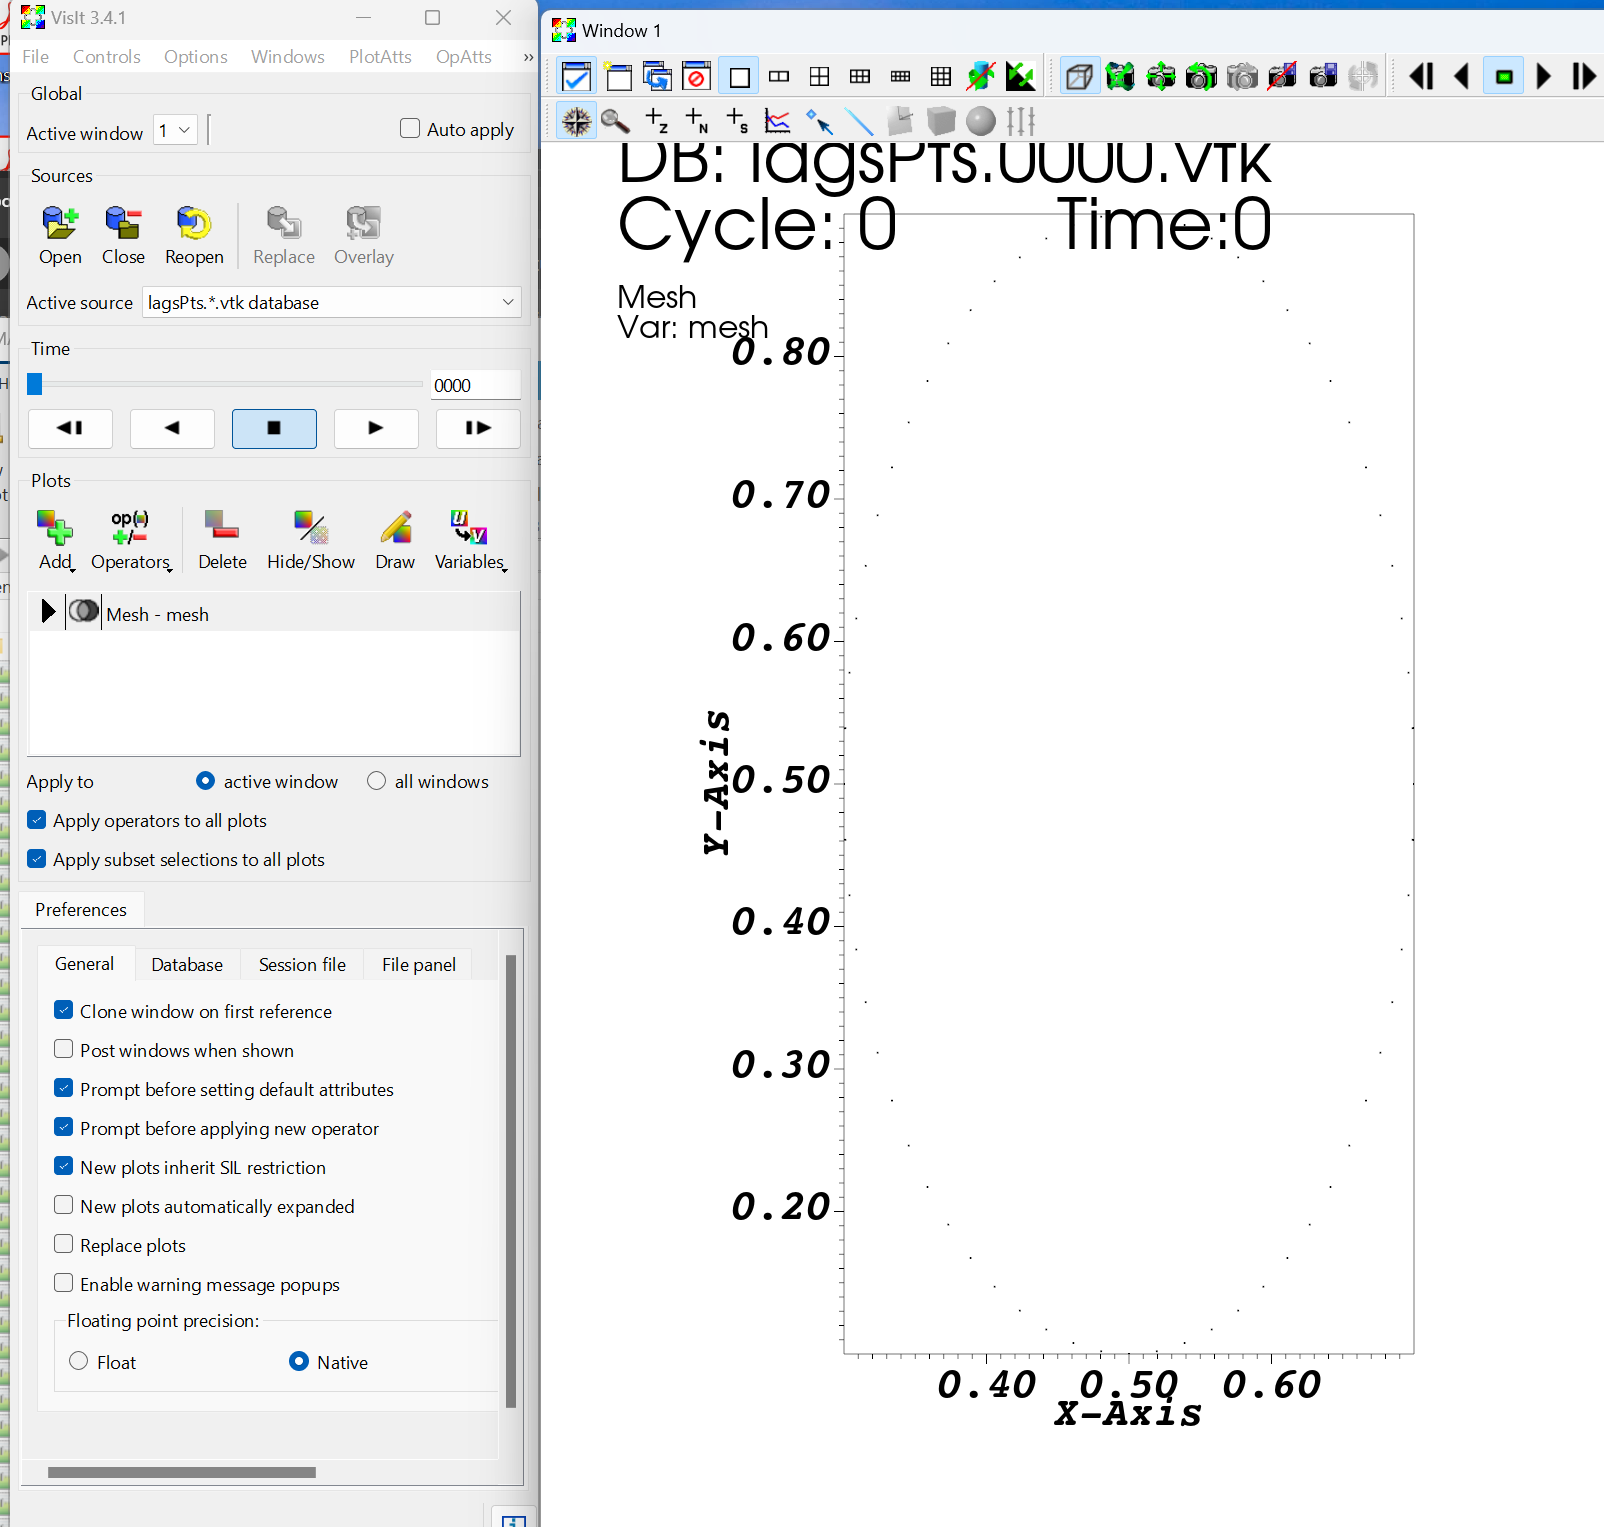
\includegraphics[width=\linewidth,height=0.78\textheight,keepaspectratio]{ch26-gui-main.png}
\column{0.56\textwidth}
\footnotesize
\begin{itemize}
  \item \gui{Sources}: \gui{Open} a database; the \gui{Active source} is the one new plots read from. Two databases in one window is the normal state for an IBAMR run.
  \item \gui{Time}: the slider and the play buttons; one slider steps all correlated sources.
  \item \gui{Plots}: \gui{Add} a plot of a variable of the active source, \gui{Operators}, \gui{Delete}, \gui{Hide/Show}, \gui{Draw}, \gui{Variables}; the list shows \code{database:Plot -- variable}; double-clicking a line opens its attribute window.
  \item Below the list: the attribute window of the selected plot (or the Preferences, as in the picture) docks here in 3.x; the 2.x decks had it floating.
  \item \gui{Controls} menu: Annotation, Color table, Database correlations, Expressions, Query, Pick, Subset, View. \gui{File}: Save window, Set save options, Save movie, Save/Restore session.
\end{itemize}
\sourcecredit{VisIt 3.4.1 on Windows, the IB2d rubber band (2024 practical, slide 16). The 3.5 window is identical.}
\end{columns}
\end{frame}

% 7
\begin{frame}{Set one preference first}
\label{fr:prefs}
\begin{columns}[T]
\column{0.5\textwidth}
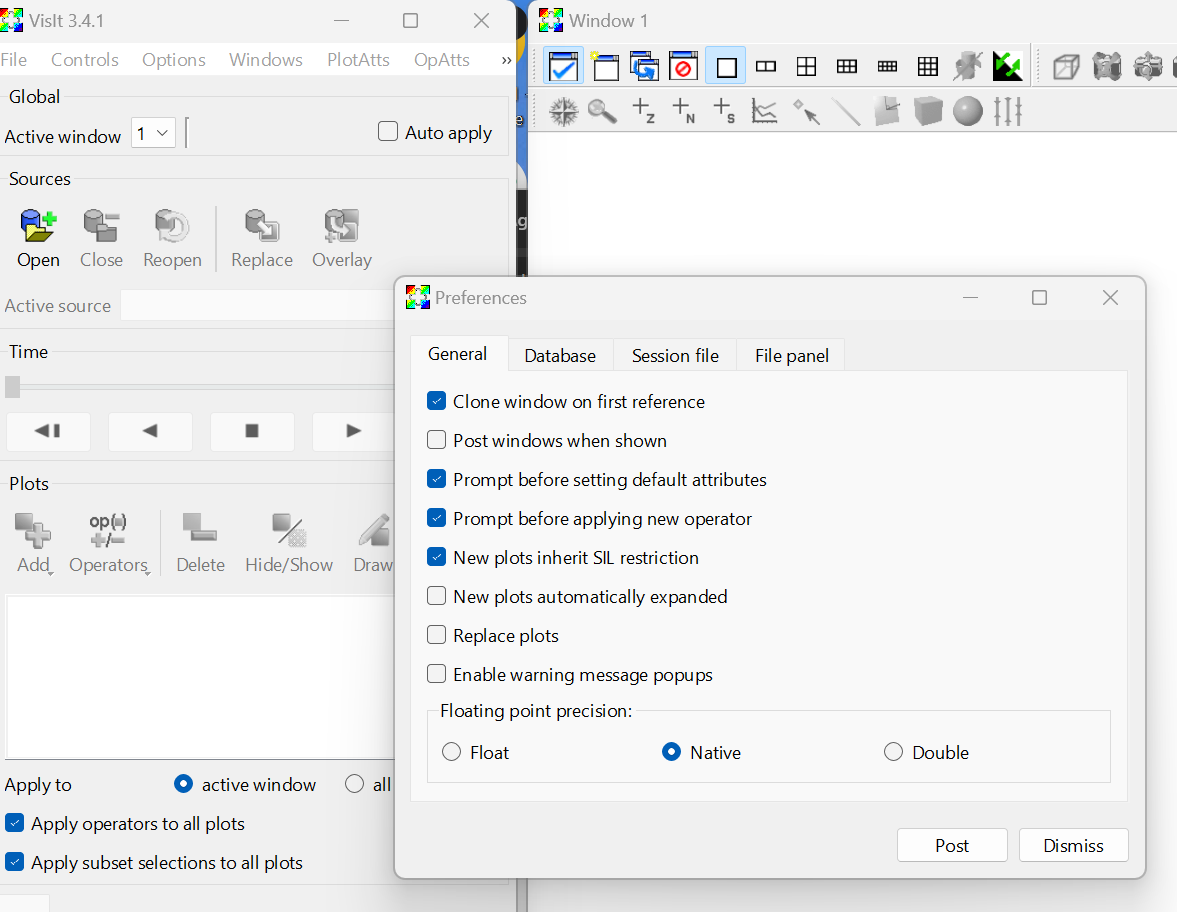
\includegraphics[width=\textwidth]{ch26-gui-prefs.png}
\column{0.48\textwidth}
\footnotesize
\begin{itemize}
  \item \gui{Options $\to$ Preferences} (3.x; on the Mac of the 2020 deck it was under the \gui{VisIt 2.5.2} application menu): untick \gui{Enable warning message popups}, \gui{Apply}.
  \item Every one of the old decks starts here, for a reason: when a movie is saved frame by frame a warning box can appear at every frame and stop the loop until it is dismissed.
  \item \gui{Auto apply} (top of the main window) applies attribute changes without the \gui{Apply} button: handy while tuning, slow on large data.
  \item The other tabs: \gui{Database} (``Try harder to get cycles and times'' when the time annotation shows frame indices instead of times), \gui{Session file}, \gui{File panel}.
\end{itemize}
\sourcecredit{VisIt 3.4.1 (2024 practical, slide 12).}
\end{columns}
\end{frame}

% 8
\begin{frame}{Open the points, add the mesh, draw}
\label{fr:open}
\begin{columns}[T]
\column{0.5\textwidth}
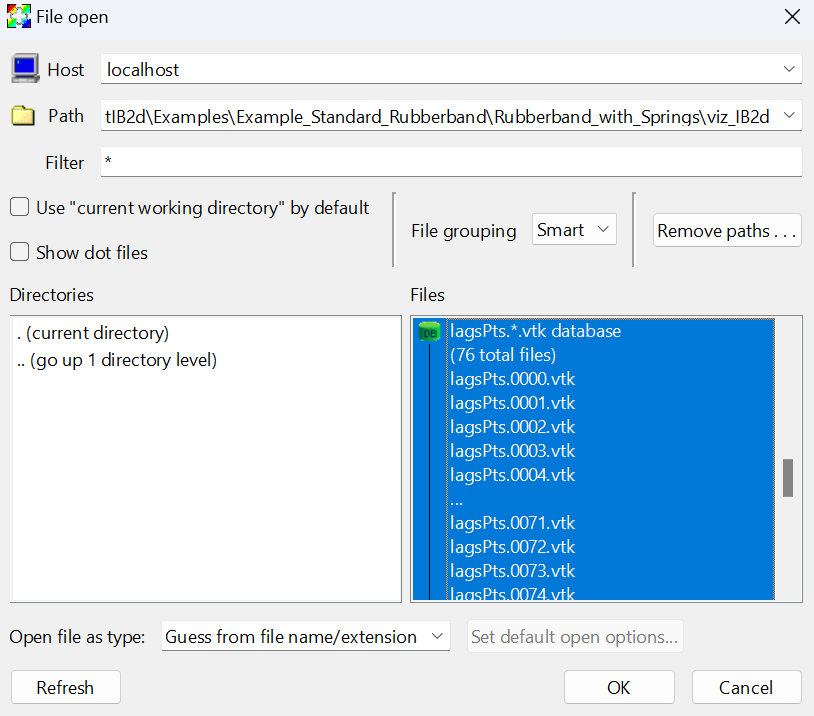
\includegraphics[height=0.44\textheight]{ch26-gui-open.png}\hspace{1mm}
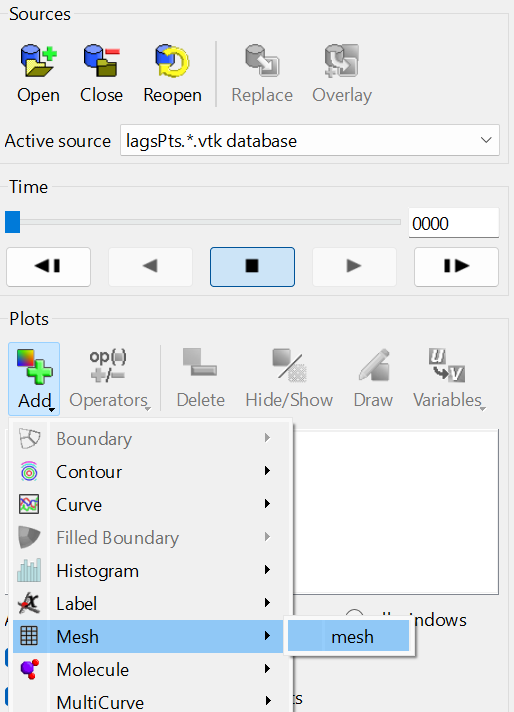
\includegraphics[height=0.44\textheight]{ch26-gui-add-mesh.png}
\column{0.48\textwidth}
\scriptsize
\begin{enumerate}
  \item \gui{Open}, go to the run's \code{viz\_IB2d} folder, choose \code{lag\_data.visit}. VisIt reads the first frame and lists what it holds; the window stays blank: opening is not drawing.
  \item \gui{Add $\to$ Mesh $\to$ human\_vertices} (the structure name from your \code{input2d}; the 2024 picture shows IB2d's single \code{mesh}), then \gui{Draw}. The points appear, tiny, in the default colour.
  \item Double-click the plot line, or select it and look below the list: the \gui{Mesh} attributes (next slide).
  \item The 2020 and 2024 decks both say ``nothing has shown up'' between steps 1 and 2: it is the single most common first question.
\end{enumerate}
\sourcecredit{VisIt 3.4.1 (2024 practical, slides 13--14): the File open dialog with a \code{.vtk} series grouped as one database, and the Add menu.}
\end{columns}
\end{frame}

% 9
\begin{frame}{The first picture, and the Mesh attributes}
\label{fr:points}
\centering
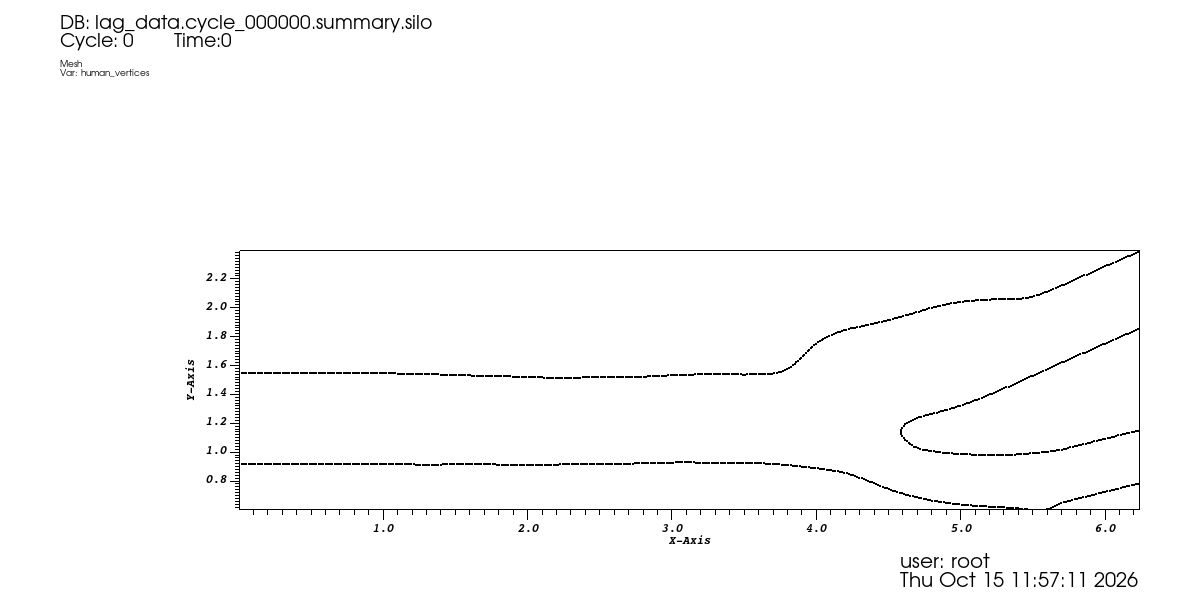
\includegraphics[height=0.5\textheight]{ch26-1-points-default.png}\hspace{2mm}
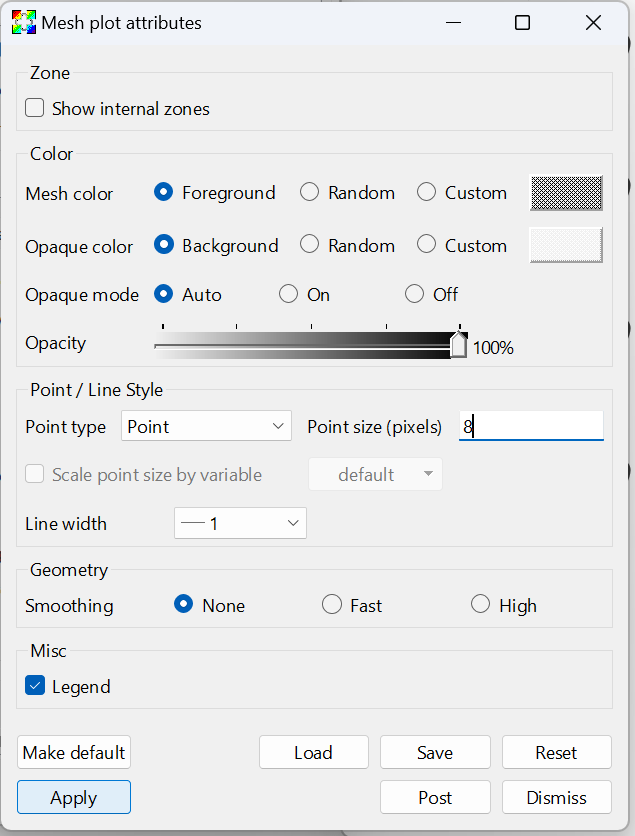
\includegraphics[height=0.5\textheight]{ch26-gui-mesh-attr.png}\\[1mm]
\scriptsize\raggedright
Left: the Mesh plot of \code{human\_vertices} as VisIt first draws it, with the default annotations (axes, the database name top left, the user name and date bottom right, a legend). Right: the Mesh plot attributes (3.4.1; the same in 3.5): \gui{Mesh color} \gui{Custom} (black), \gui{Point type} Point or Sphere, \gui{Point size (pixels)} 4--8 for a figure, \gui{Line width} 2--4 when the plot is \code{<name>\_mesh}, the spring mesh, whose edges then draw as a continuous thick line (slide \ref{fr:boundary}); \gui{Legend} off. The 2020 ``suggestions'' slide: ``when drawing the boundary, usually you want to plot the vertices; increase the pixel size to make lines larger.''
\end{frame}

% 10
\begin{frame}{Open the fluid: the plot VisIt adds by itself}
\label{fr:dumps}
\begin{columns}[T]
\column{0.52\textwidth}
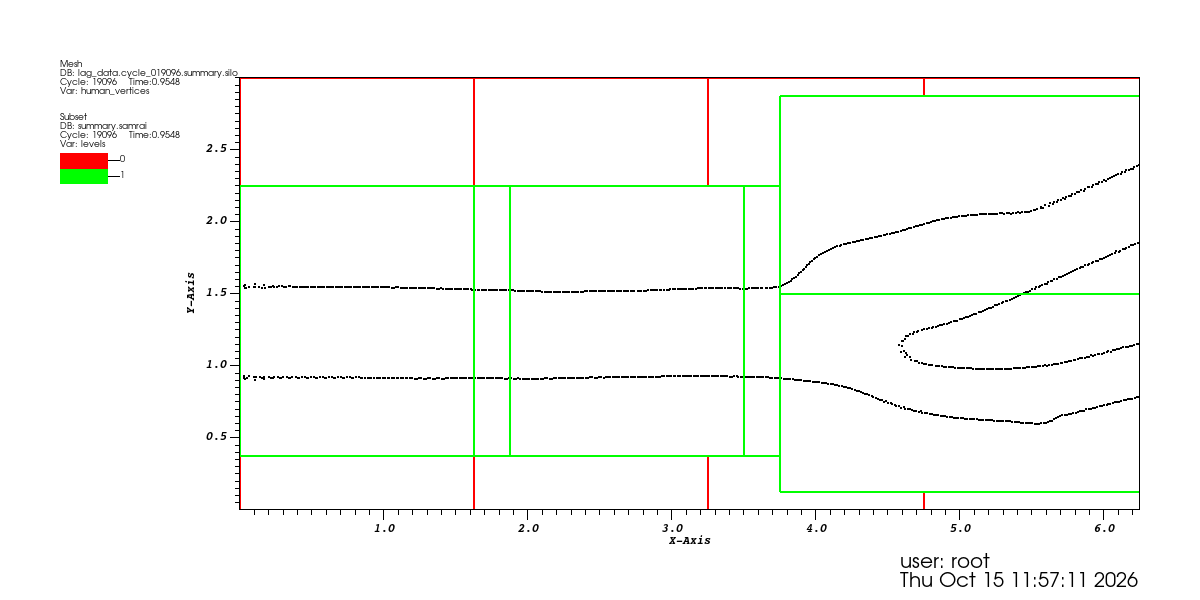
\includegraphics[width=\textwidth]{ch26-2-levels-auto.png}
\column{0.46\textwidth}
\scriptsize
\begin{itemize}
  \item \gui{Open} again, choose \code{dumps.visit}. VisIt asks whether to create a \emph{database correlation} between the two sources: say yes (slide \ref{fr:time}). The active source is now \code{dumps.visit}.
  \item Then, unasked, a plot appears: \code{dumps.visit:Subset -- levels}, the refinement levels as coloured boxes (red level 0, green level 1 here). A SAMRAI database declares it as its default plot and VisIt draws it on open. The 2020 deck: ``these boxes will get in the way, so click Hide/Show to hide them''; deleting it is cleaner (\gui{Delete} with the line selected), because a hidden plot still saves its legend.
  \item The same boxes are useful once: they show where the fine level sits and that it follows the body (slide \ref{fr:amr}).
\end{itemize}
\sourcecredit{VisIt 3.5.0, headless, IB/13 human at $t = 0.95$ s: the Mesh plot of the points and the Subset plot that appeared on opening the dumps.}
\end{columns}
\end{frame}

% 11
\begin{frame}{Plot the vorticity}
\label{fr:omega}
\begin{columns}[T]
\column{0.5\textwidth}
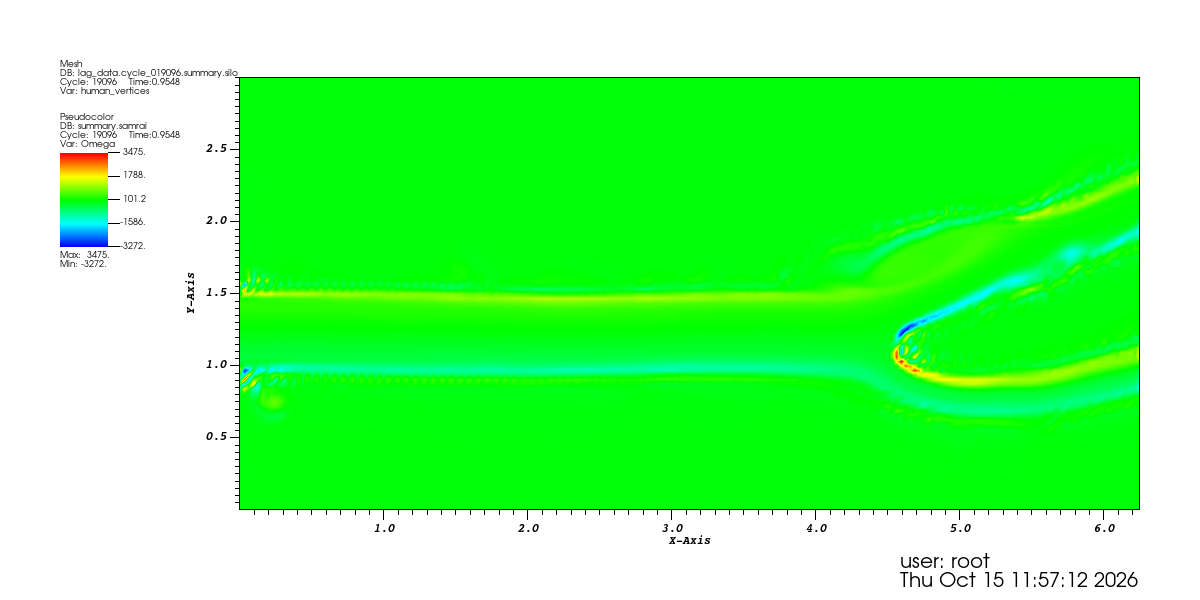
\includegraphics[width=\textwidth]{ch26-2-omega-default.png}
\column{0.48\textwidth}
\footnotesize
\begin{enumerate}
  \item With \code{dumps.visit} active, \gui{Add $\to$ Pseudocolor $\to$ Omega}, \gui{Draw}. Plots draw in the order they were added, so a Pseudocolor added after the points hides them (the 2024 practical re-adds the mesh on top; lowering the Pseudocolor's opacity also works).
  \item At frame 0 the fluid is at rest and the picture is blank, which the 2015 deck recorded as ``Vector plot yielded no data at $t = 0$''. Move the slider; the picture is frame 56 of 102, the systolic peak of the second cycle.
  \item The default colour map (\code{hot}) runs from the frame's minimum to its maximum, so every frame has its own scale and the wall vorticity ($\pm3000$ s$^{-1}$) saturates everything: green with two thin streaks. The next slide fixes it.
\end{enumerate}
\sourcecredit{VisIt 3.5.0, headless, IB/13 human: the Pseudocolor of \code{Omega} as first drawn.}
\end{columns}
\end{frame}

% 12
\begin{frame}{Pseudocolor attributes}
\label{fr:pcattr}
\begin{columns}[T]
\column{0.44\textwidth}
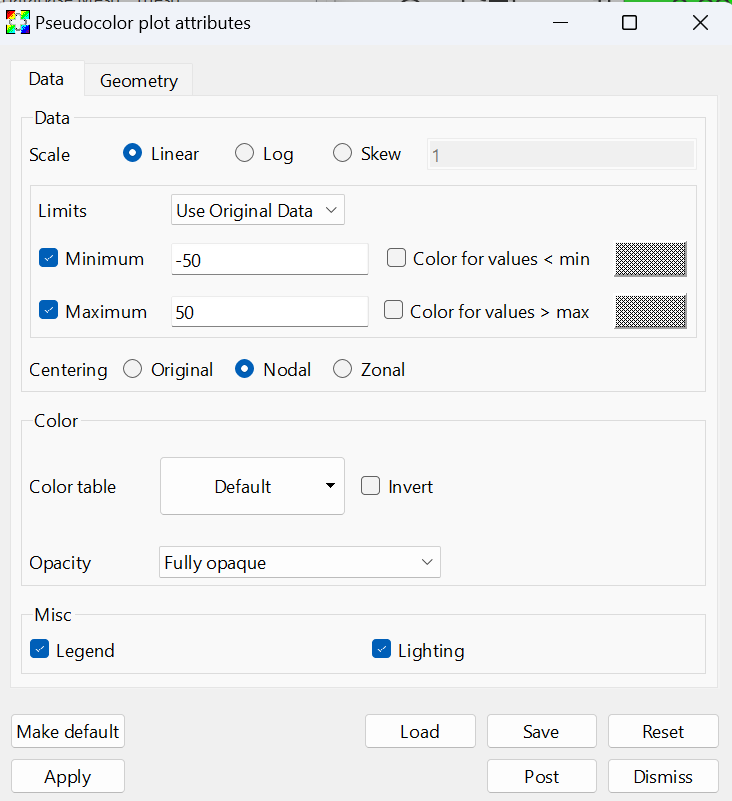
\includegraphics[width=0.48\linewidth,height=0.66\textheight,keepaspectratio]{ch26-gui-pc-attr.png}\hfill
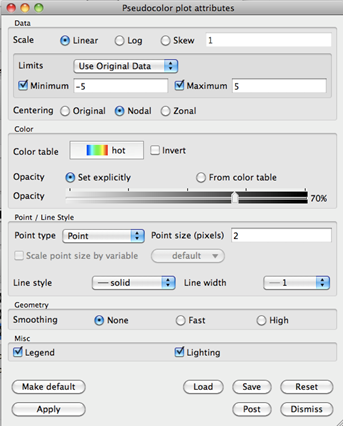
\includegraphics[width=0.48\linewidth,height=0.66\textheight,keepaspectratio]{ch26-v2-pc-attr.png}
\column{0.54\textwidth}
\scriptsize
\begin{itemize}
  \item \gui{Data} tab. \gui{Limits}: tick \gui{Minimum} and \gui{Maximum} and type them. The 2020 rule: look at the automatic range once, then set a quarter of it or less, so the walls saturate and the vortices in the stream show: $\pm300$ s$^{-1}$ here, for extremes of $\pm3000$.
  \item \gui{Centering}: \gui{Nodal}. The dumps are cell values; nodal centering averages them to the corners and the plot is smooth instead of blocky (2020: ``reduces the noisiness around the boundaries'').
  \item \gui{Color table}: \code{difference} (blue--white--red, zero in the middle) for a signed field; \code{viridis} or \code{hot} for a magnitude (slide \ref{fr:ctable}).
  \item \gui{Opacity}: 70\% lets vectors drawn on top read through (2020); fully opaque for a figure without vectors.
  \item \gui{Apply}; the attributes stay with the plot for every frame and in the session.
\end{itemize}
\end{columns}
\sourcecredit{Left: VisIt 3.4.1 (2024, slide 22; limits $\pm50$ for the rubber band). Right: the same window in 2.5.2 (2020, slide 13; limits $\pm5$, \code{hot}, 70\%).}
\end{frame}

% 13
\begin{frame}{Before and after}
\label{fr:beforeafter}
\centering
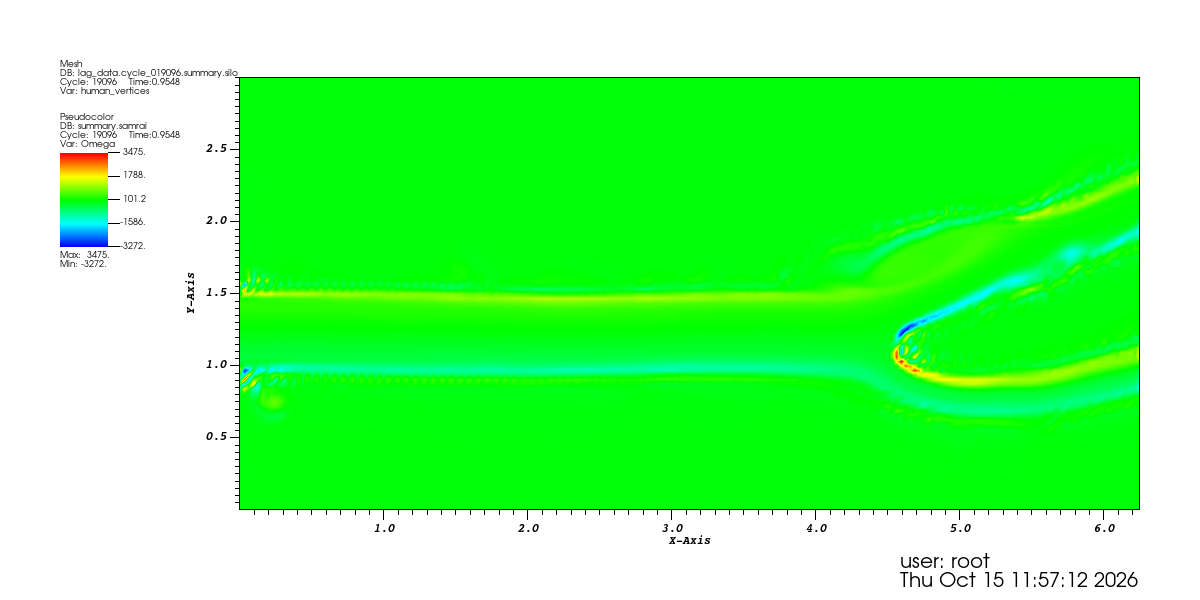
\includegraphics[width=0.48\textwidth]{ch26-2-omega-default.png}\hfill
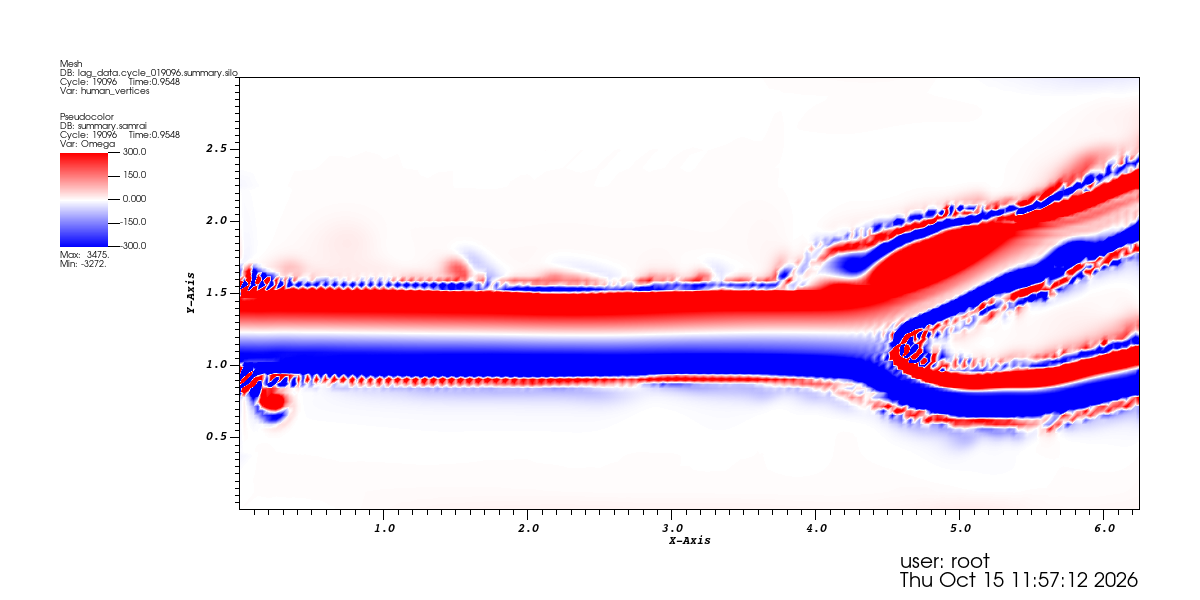
\includegraphics[width=0.48\textwidth]{ch26-3-omega-tuned.png}\\[1mm]
\scriptsize The same frame (the systolic peak of the second cycle, $t = 0.95$ s): automatic limits, zonal, \code{hot} on the left; $\pm300$ s$^{-1}$, nodal, \code{difference}, 70\% opacity on the right. Nothing in the data changed. The default annotations are still on in both: the database names and times top left, the user name and date bottom right, a legend with \gui{Max}/\gui{Min} lines (slide \ref{fr:annot}).
\end{frame}

% 14
\begin{frame}{The time slider and the database correlation}
\label{fr:time}
\centering
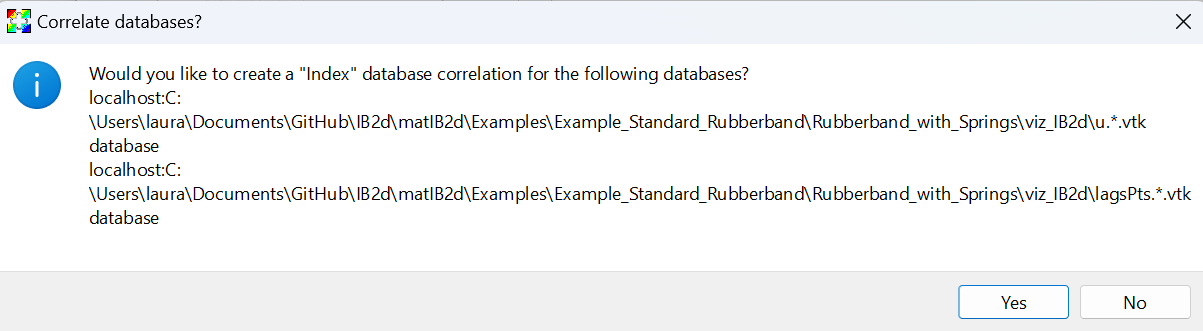
\includegraphics[width=0.66\textwidth]{ch26-gui-correlate.png}\\[1mm]
\scriptsize\raggedright
\begin{itemize}
  \item The prompt appears when a second time-varying database is opened (or, in the 2024 practical, when the first plot of it is added): say \gui{Yes}. The \gui{Time} panel then shows \gui{Active time slider: Correlation01}, and \gui{Play}, the single-step arrows and the slider move both sources together, because they have the same number of frames.
  \item If you said \gui{No}, each source has its own slider and the points stay at frame 0 while the fluid moves: the classic ``the boundary doesn't move'' question. \gui{Controls $\to$ Database correlations} makes or edits a correlation later, by index or by time.
  \item The frame index is not the time: \gui{Controls $\to$ Annotation $\to$ General} shows the cycle and time taken from the dumps, but only on the database's line (``Cycle: 32000\ \ Time:1.6'' under ``DB: \dots''); for the time alone, a text annotation with \code{\$time} (chapter 30).
  \item A correlation by index assumes equal intervals. If the two \code{*\_dump\_interval} values differ, correlate by time, or fix the input. Rendering every frame is what makes a movie (chapter 30); for a figure, stop at the frame you want and save the window.
\end{itemize}
\sourcecredit{VisIt 3.4.1 (2024 practical, slide 18; the IB2d paths).}
\end{frame}

% 15
\begin{frame}{Vectors}
\label{fr:vectors}
\begin{columns}[T]
\column{0.42\textwidth}
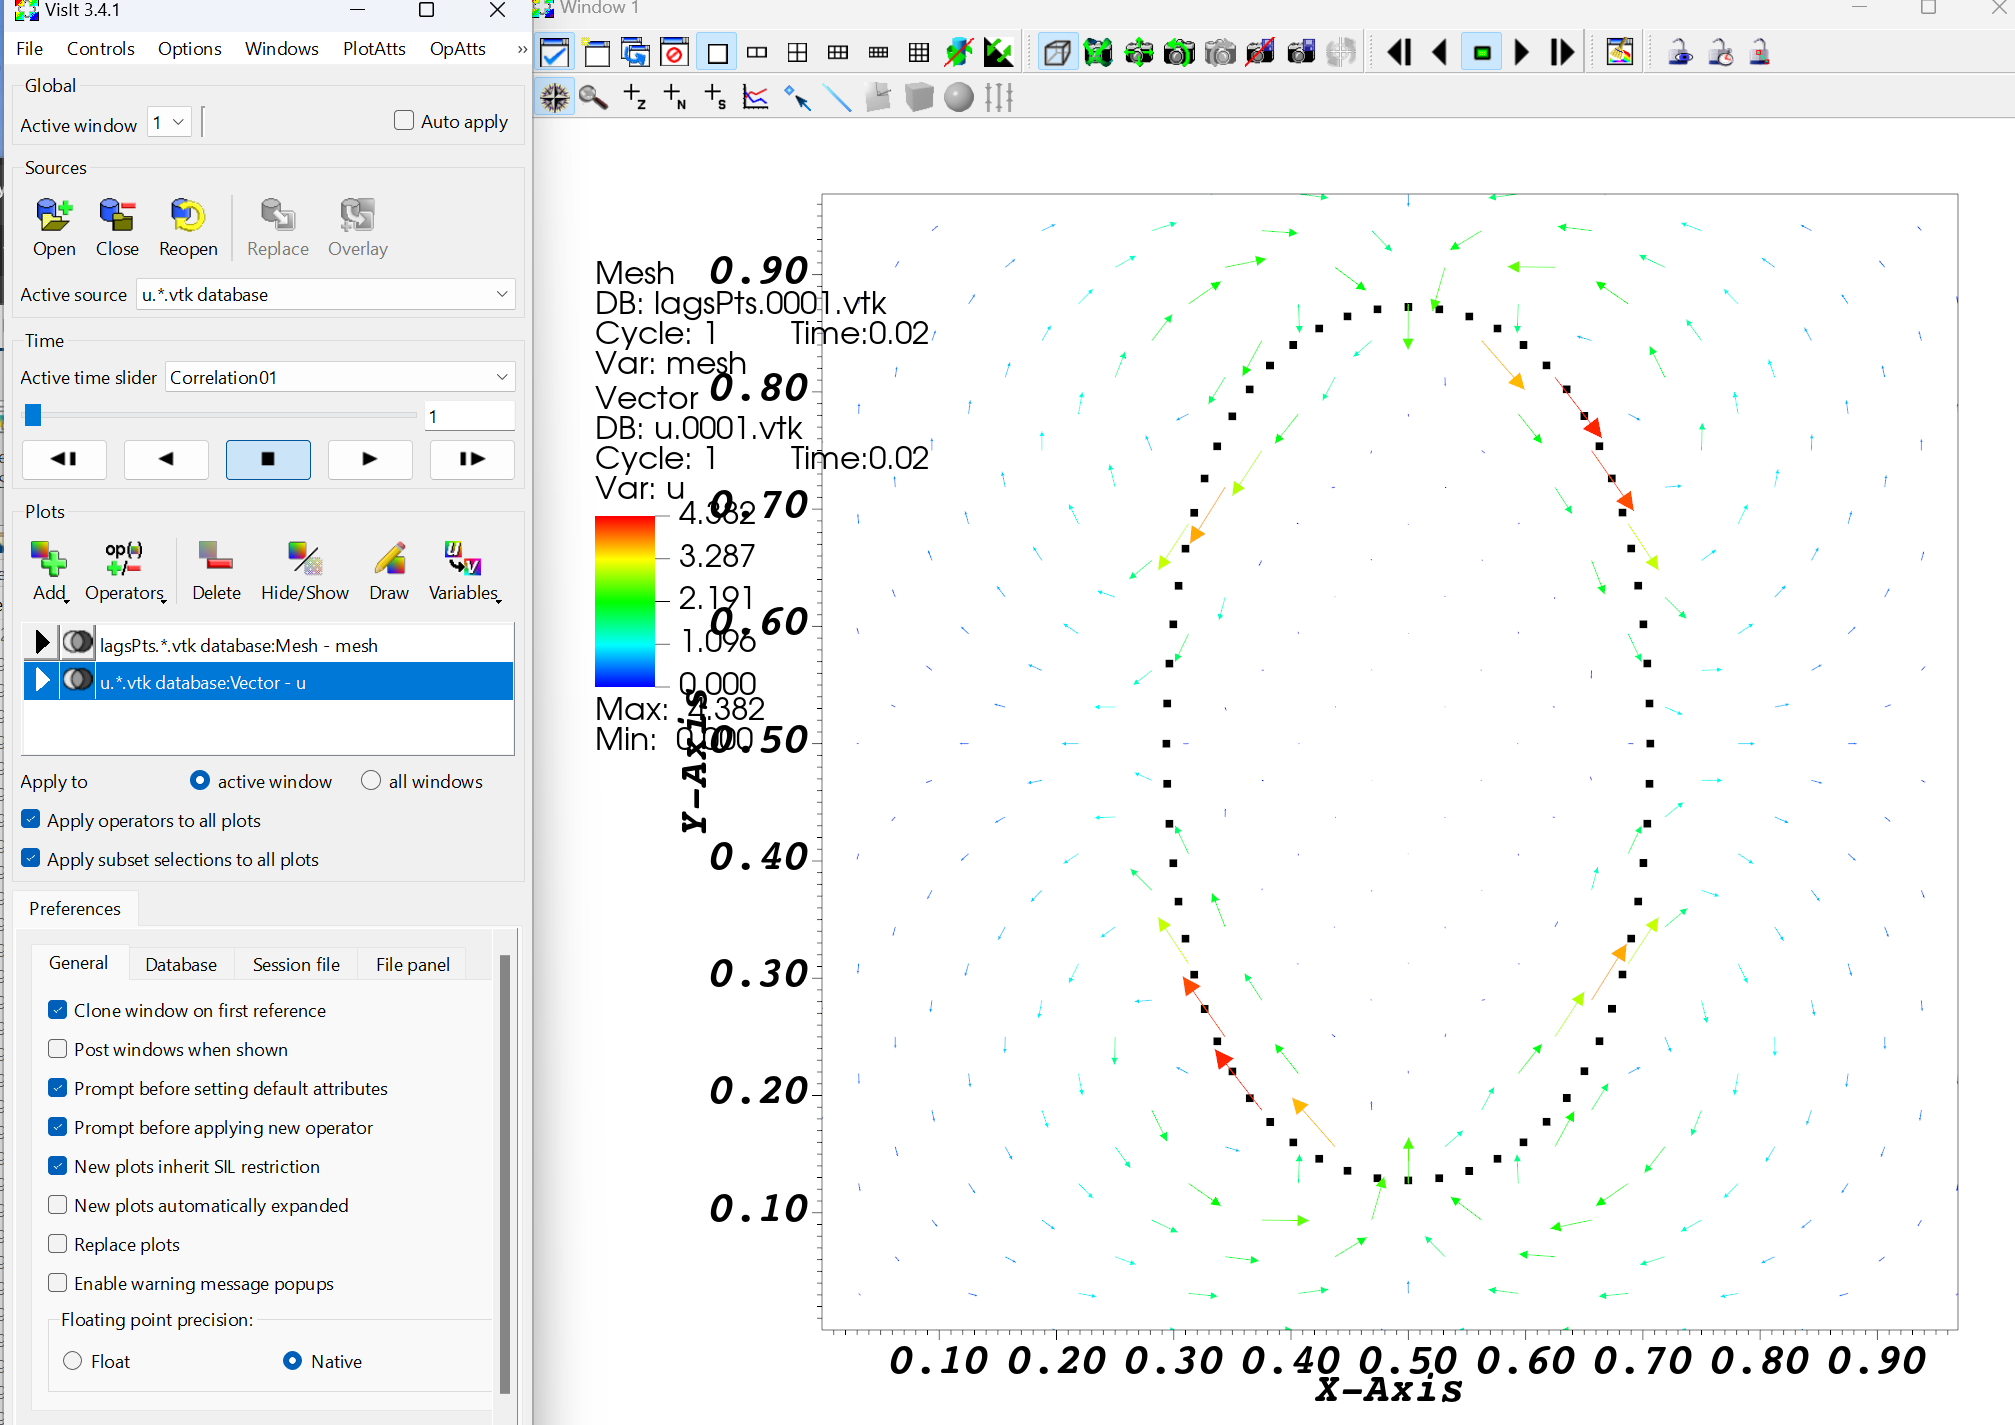
\includegraphics[width=\textwidth]{ch26-gui-vectors-ib2d.png}
\column{0.56\textwidth}
\scriptsize
\begin{itemize}
  \item \gui{Add $\to$ Vector $\to$ U}, \gui{Draw}: one arrow per cell, coloured by magnitude, scaled automatically: a hedgehog (left, on the IB2d rubber band at its first frame). Its attribute window fixes it (next slide).
  \item From VisIt 3.2 on the Vector window has the \gui{Sampling}, \gui{Data} and \gui{Geometry} tabs (3.0--3.1: \gui{Vectors}, \gui{Data}, \gui{Glyphs}); the 2020 deck's \gui{Location}, \gui{Form} and \gui{Rendering} are the 2.5.2 names of the same controls.
  \item \gui{Placement}: uniform throughout the mesh (not one per cell, which crowds the fine AMR levels) and a \gui{Fixed number}: the 2020 deck said 8000, the 2014 one 12000; 3000--5000 reads at slide size.
  \item \gui{Scale}: untick \gui{Auto scale}, set \gui{Scale} so the longest arrow spans a few cells; tick \gui{Scale by magnitude} so arrow length means speed (the 2018 correction of the 2014 deck's scale, 0.4 for 0.04, is this knob). \gui{Head size} about 0.25.
  \item \gui{Color}: \gui{Constant} (black or dark grey) when the arrows sit on a colour map, so that ``the colours of the two plots do not fight'' (2020). The plot's own \gui{Legend} tick turns its colour bar off.
\end{itemize}
\sourcecredit{VisIt 3.4.1 (2024 practical, slide 19).}
\end{columns}
\end{frame}

% 16
\begin{frame}{The Vector window, then and now}
\label{fr:vectabs}
\centering
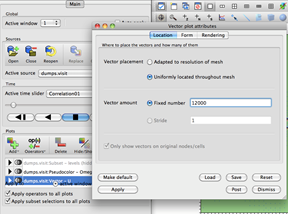
\includegraphics[height=0.38\textheight]{ch26-v2-vec-location.png}\hfill
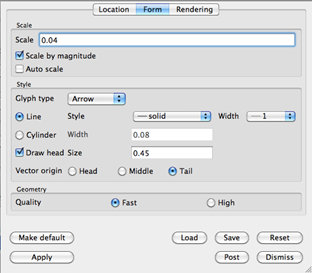
\includegraphics[height=0.38\textheight]{ch26-v2-vec-form.png}\hfill
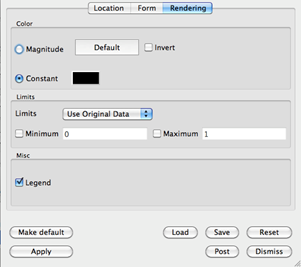
\includegraphics[height=0.38\textheight]{ch26-v2-vec-rendering.png}\\[1mm]
\scriptsize\raggedright
\begin{tabular}{@{}L{0.22\textwidth}L{0.42\textwidth}L{0.26\textwidth}@{}}
\toprule
2.5.2 tab (above) & what it holds & 3.5 tab \\
\midrule
\gui{Location} & placement (adapted to the mesh / uniform), fixed number or stride & \gui{Sampling} \\
\gui{Form} & scale, scale by magnitude, auto scale, glyph type, line width, head size, origin & \gui{Geometry} \\
\gui{Rendering} & colour by magnitude or constant, limits, legend & \gui{Data} \\
\bottomrule
\end{tabular}
\sourcecredit{VisIt 2.5.2 (2020 deck, slides 16--18): 12000 vectors, scale 0.04 (corrected to 0.4 in 2018), head 0.45, constant black. The values this chapter uses: 4000, scale by magnitude with the scale set by eye, head 0.25, black.}
\end{frame}

% 17
\begin{frame}{Vectors on the vorticity, and the zoom}
\label{fr:vecpic}
\centering
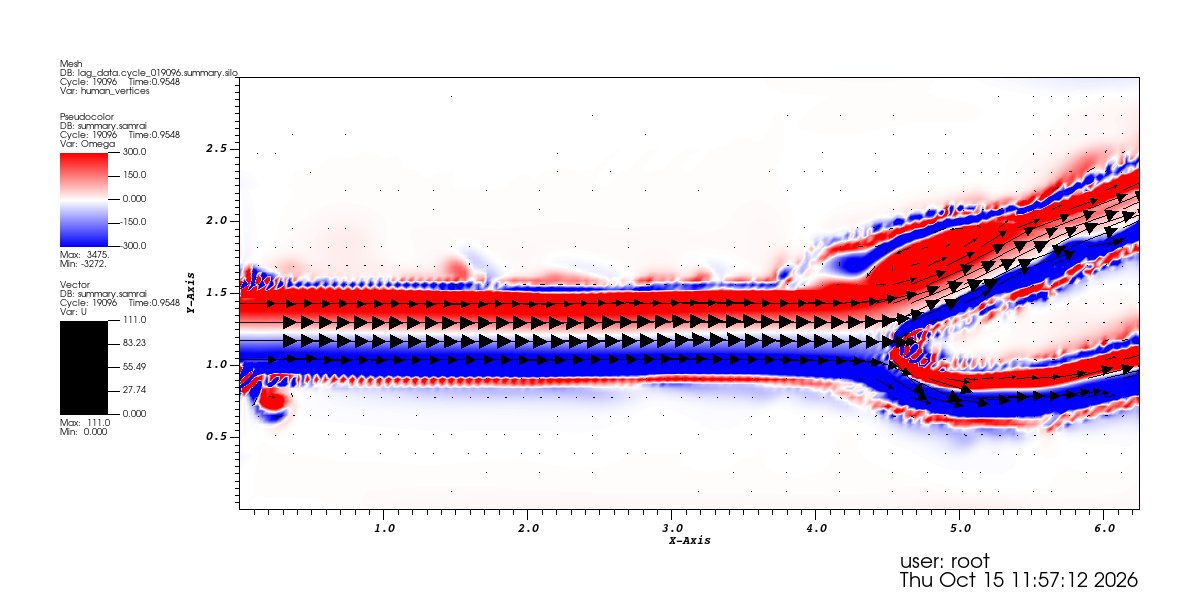
\includegraphics[width=0.48\textwidth]{ch26-4-vectors.png}\hfill
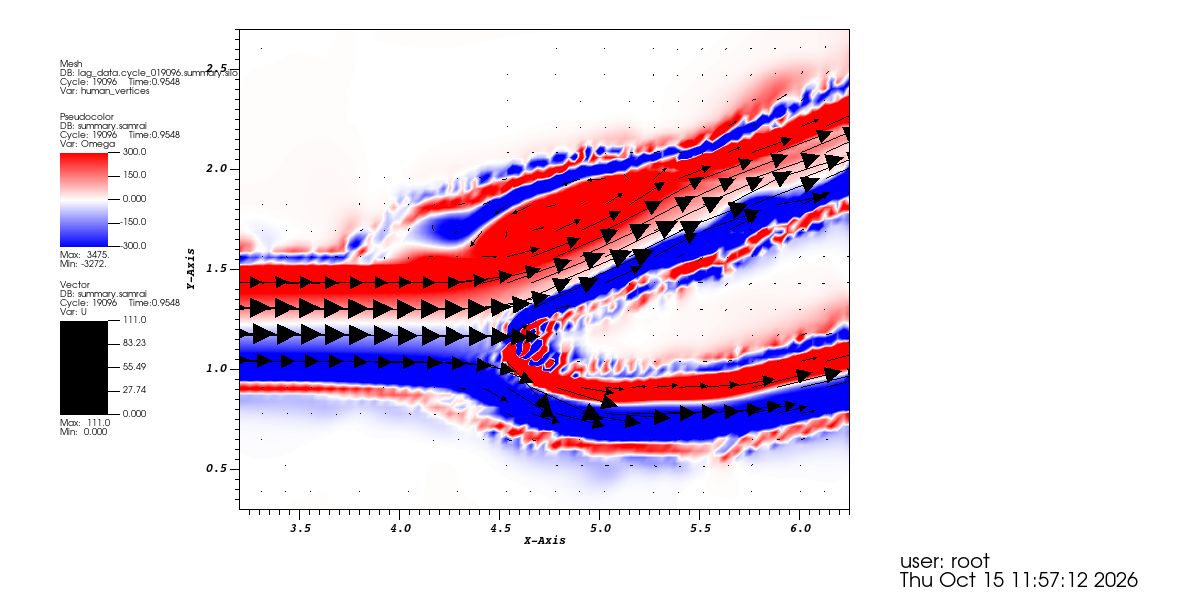
\includegraphics[width=0.48\textwidth]{ch26-5-zoom.png}\\[1mm]
\scriptsize\raggedright Left: 4000 uniformly placed vectors in black over the vorticity at 70\% opacity. Right: zoomed to the bifurcation by dragging a box in the window (the \gui{Zoom} mode, the magnifier in the toolbar); the camera with the green cross, or \gui{View $\to$ Reset view}, undoes it. \gui{Controls $\to$ View} types the window coordinates exactly (the CLI's \code{windowCoords}; here $3.2 \le x \le 6.25$, $0.3 \le y \le 2.7$ cm), which is how a figure is reproduced.
\end{frame}

% 18
\begin{frame}{The AMR grid: Subset plots and the mesh}
\label{fr:amr}
\begin{columns}[T]
\column{0.6\textwidth}
\footnotesize
\begin{itemize}
  \item \gui{Add $\to$ Subset $\to$ levels} colours each refinement level (the plot of slide \ref{fr:dumps}, added by VisIt itself); \gui{Subset $\to$ patches} colours each patch; \gui{Add $\to$ Mesh $\to$ amr\_mesh} draws every cell. The 2015 lecture used the first two to show where the fine grid sits and that it follows the body.
  \item A Subset plot is also how you \emph{hide} a level: the Subset window (\gui{Controls $\to$ Subset}) unticks levels or patches for every plot, which is how a coarse-level-only picture is made.
  \item The coloured straight lines that turn up in saved pictures of IBAMR runs are this plot, forgotten in the list or merely hidden (a hidden plot keeps its legend); delete it. Chapter 30's frame cleaner (\code{examples/analysis/movie\_clean.py}) removes such lines after the fact, for pictures made before the cause was known.
  \item \gui{Operators $\to$ Selection $\to$ Box} restricts every plot to a box (chapter 29 uses it for queries); \gui{Operators $\to$ Transforms $\to$ Reflect} mirrors a half-domain run.
\end{itemize}
\column{0.38\textwidth}
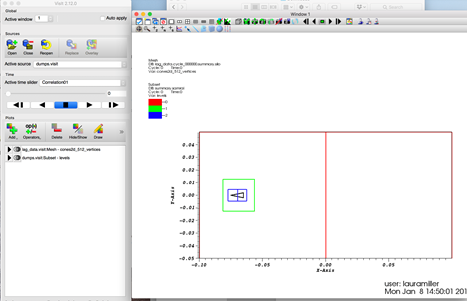
\includegraphics[width=\textwidth]{ch26-v2-levels.png}
\sourcecredit{VisIt 2.5.2 (2020 deck, slide 10): \code{dumps.visit:Subset -- levels} as it appeared on open, with the 2014 flow-past-a-triangle data.}
\end{columns}
\end{frame}

% 19
\begin{frame}[fragile]{Variables and expressions}
\label{fr:expr}
\footnotesize
\begin{columns}[T]
\column{0.5\textwidth}
\begin{lstlisting}[style=tiny]
# Controls > Expressions: name, type, definition
Umag      scalar   magnitude(U)
u         scalar   U[0]
v         scalar   U[1]
speed_cm  scalar   100*magnitude(U)       # a unit change
omega_abs scalar   abs(Omega)
dX        vector   {dX_0, dX_1}           # IBFE only: the Exodus file's displacement (ch. 28)
\end{lstlisting}
\begin{center}
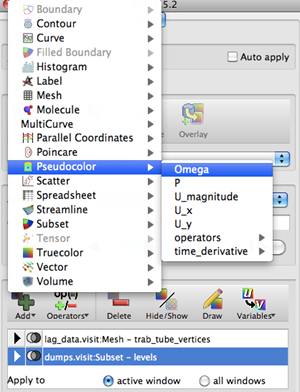
\includegraphics[height=0.2\textheight]{ch26-v2-pc-menu.png}
\end{center}
\sourcecredit{VisIt 2.5.2 (2020 deck, slide 11): the Pseudocolor menu then listed \code{Omega}, \code{P}, \code{U\_magnitude}, \code{U\_x}, \code{U\_y}; 0.19 writes the vector \code{U} and leaves the rest to expressions.}
\column{0.48\textwidth}
\scriptsize
\begin{itemize}\setlength{\itemsep}{-0.5pt}
  \item An expression is a new variable, computed from the others when a plot asks for it; it appears in the \gui{Add} menus under its type. \code{U[0]} and \code{U[1]} are the components, \code{magnitude(U)} the speed; the Vector plot takes \code{U} itself.
  \item \code{Omega} is a scalar in 2D and a vector in 3D (\code{Omega[2]} for the spanwise component, chapter 27).
  \item \code{P} is the pressure with the mean removed when \code{normalize\_pressure = TRUE}, and relative to the outflow when it is \code{FALSE} (IB/13): a Pseudocolor of \code{P} has no absolute meaning in the first case.
  \item \code{Div U} should be at round-off: a Pseudocolor of it is the first health check of a run (chapter 16).
  \item The Silo files of a point-method run carry the positions only (no velocity, force or displacement: those are the \code{hier\_data} files of chapter 11); a displacement since the first frame can still be built as a cross-time expression (chapter 28). The \code{dX\_0}, \code{dX\_1} fields belong to the ExodusII file of an IBFE run, which chapter 28 uses to displace a finite-element mesh.
  \item Expressions are saved in the session, not in the data; a session restored on another run keeps them.
\end{itemize}
\end{columns}
\end{frame}

% 20
\begin{frame}{Pick, Label, Spreadsheet: reading numbers off the picture}
\label{fr:pick}
\footnotesize
\begin{itemize}
  \item \gui{Pick} mode (the toolbar's crosshair, or \gui{Controls $\to$ Pick}): click a point of a plot and the Pick window lists the variables there, the cell, the level and the coordinates; \gui{Do time curve} turns the picked quantity into a curve over all frames in a new window. Chapter 29 builds on this.
  \item \gui{Add $\to$ Label $\to$ Omega} writes the value in every cell: useless on a whole grid, exactly right on a zoomed patch when you want to see what a cell holds.
  \item \gui{Add $\to$ Spreadsheet $\to$ Omega} shows the values of one patch as a table, with the patch and level chosen in its attribute window; the 2015 lecture's \code{cell\_constant} expressions and Lineouts are the other way to the numbers (chapter 29).
  \item \gui{Controls $\to$ Query}: \gui{MinMax}, \gui{Weighted variable sum}, \gui{Area}, and over time. The chapter 25 renders printed the vorticity range with \code{Query("MinMax")}, and IB/13's peak speeds came from the same query.
\end{itemize}
\end{frame}

% 21
\begin{frame}{Annotations: what a figure does not need}
\label{fr:annot}
\begin{columns}[T]
\column{0.42\textwidth}
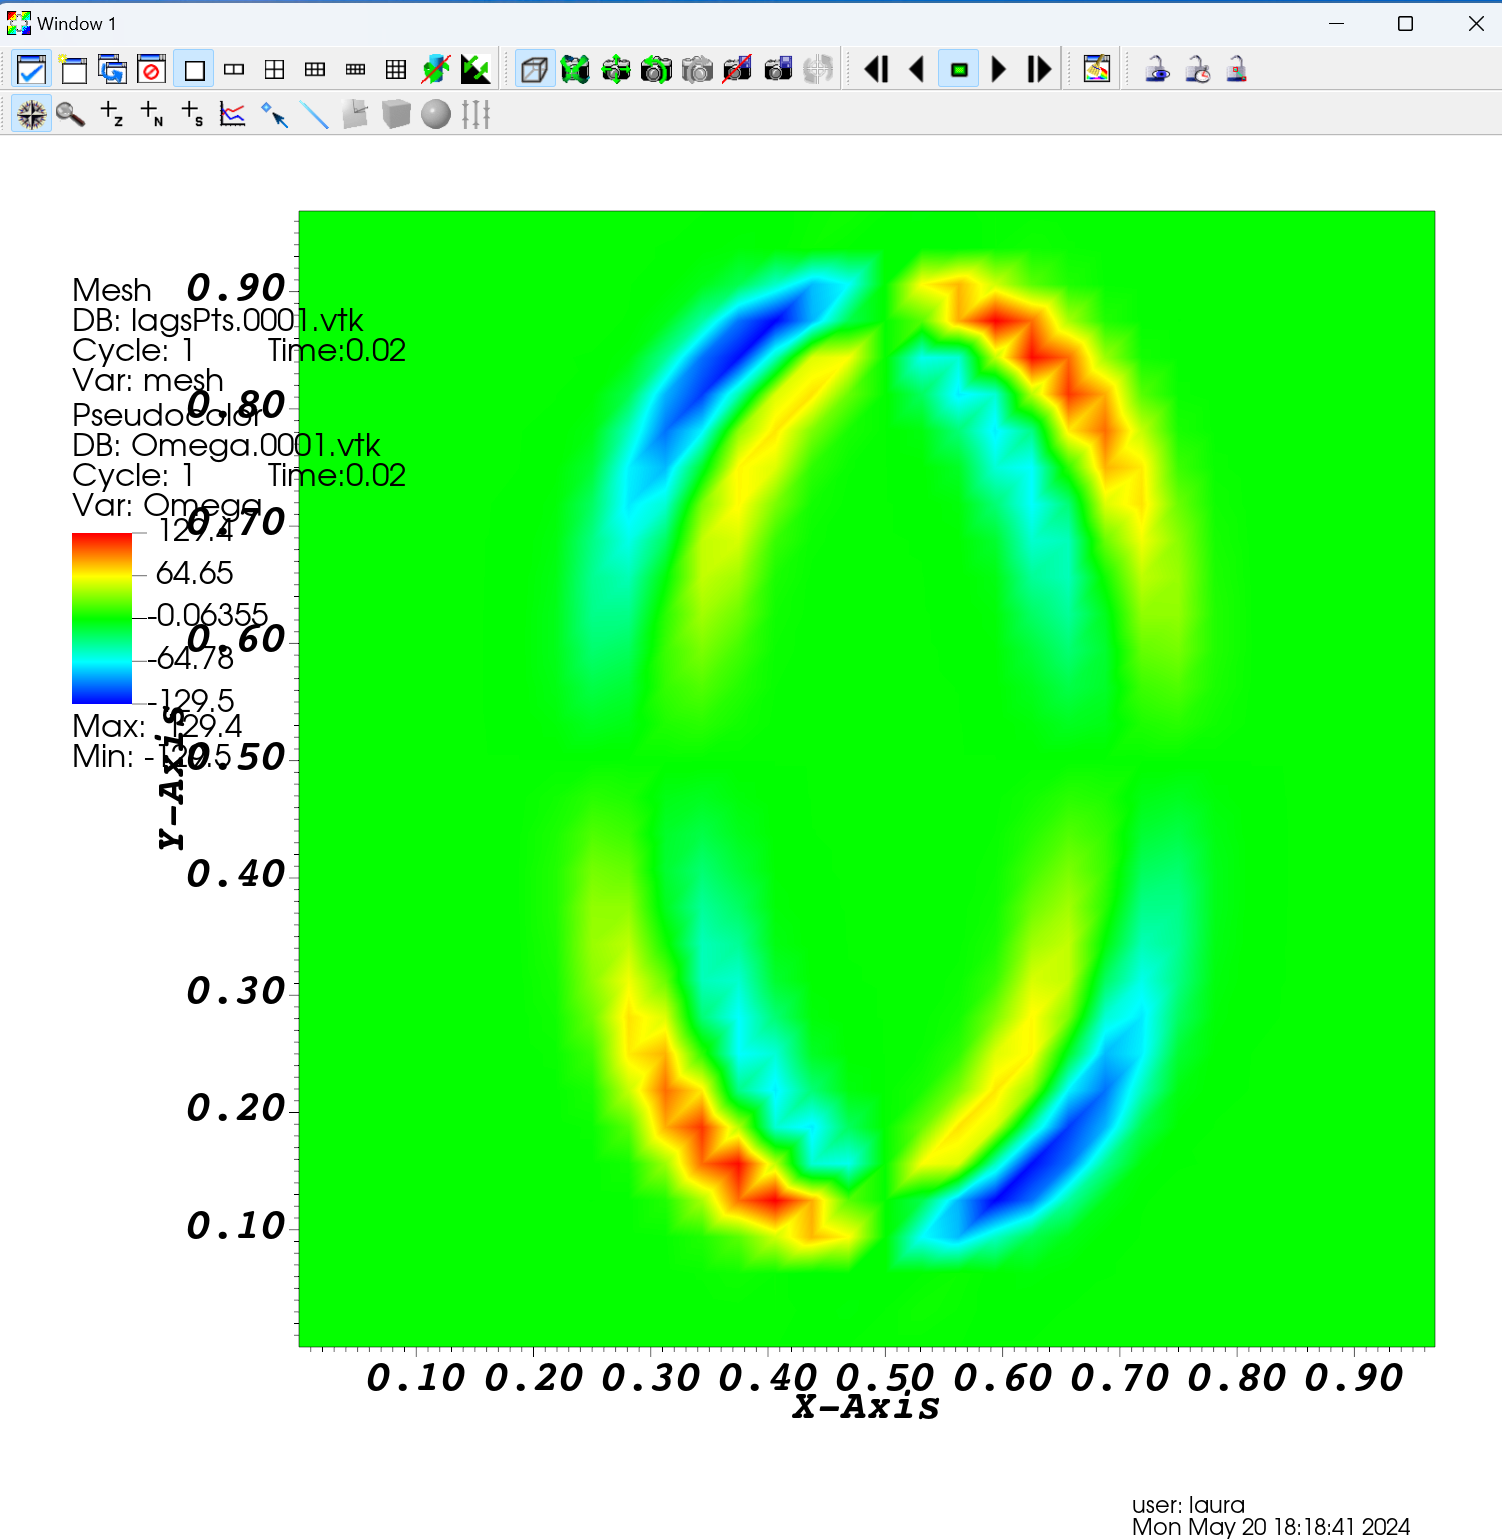
\includegraphics[width=\textwidth]{ch26-gui-pc-hides.png}
\sourcecredit{VisIt 3.4.1 (2024 practical, slide 21): everything the Annotation window turns off is on this picture.}
\column{0.56\textwidth}
\footnotesize
\begin{itemize}
  \item \gui{Controls $\to$ Annotation}. \gui{General} tab: untick \gui{User information} and \gui{Database} (the time is shown only on the database's line, so it goes too: for the frame's time add a text annotation \code{t = \$time s} in the \gui{Objects} tab, chapter 30); the \gui{Legend} tick here hides all legends at once.
  \item \gui{2D} tab: axes on or off, \gui{Custom title} and font sizes for each axis (the 2020 ``axes'' slide), tick marks and their labels, the grid lines (the 2020 ``hide the grid'').
  \item \gui{Objects} tab: the legends are objects; select one, \gui{Appearance}: untick \gui{Draw title} and \gui{Draw min/max}, set the font; \gui{Position} drags it. \gui{Create new $\to$ Text} adds a text box (the panel label, the Reynolds number), \gui{Time slider} a bar, \gui{Image} a logo.
  \item \gui{Colors} tab: background and foreground colours; a white background for print.
  \item These are window attributes, not plot attributes: they stay when plots change, and they are saved in the session.
\end{itemize}
\end{columns}
\end{frame}

% 22
\begin{frame}{The colour table}
\label{fr:ctable}
\footnotesize
\begin{itemize}
  \item \gui{Controls $\to$ Color table}: the built-in tables and their control points; \gui{New} copies one to edit; a table is chosen per plot in the plot's attributes (the \gui{Color table} button of slide \ref{fr:pcattr}). \gui{Default} on that button means the active default of this window, set here.
  \item For a signed field use a \emph{diverging} table whose middle is white or grey (\code{difference}, \code{RdBu}) with symmetric limits, so zero is the neutral colour; for a magnitude a \emph{sequential} one (\code{viridis}, \code{hot}, \code{gray}). The 2015 graph supplement's rule: it must still read in greyscale and to a colourblind reader: \code{viridis} does, the rainbow (\code{hot}, \code{rainbow}) does not.
  \item The 2013 tip, lighter-to-darker ramps of a single hue (\gui{New}, two control points), is the sequential case made by hand.
  \item \gui{Invert} flips a table; \gui{Smoothing} off makes bands, which some readers prefer for contour-like plots.
\end{itemize}
\begin{punchbox}
\scriptsize The pictures of this chapter: \code{difference} for \code{Omega} at $\pm300$ s$^{-1}$, \code{viridis} for \code{magnitude(U)} from 0 to the systolic peak.
\end{punchbox}
\end{frame}

% 23
\begin{frame}{Saving a picture}
\label{fr:save}
\begin{columns}[T]
\column{0.3\textwidth}
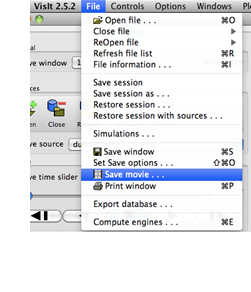
\includegraphics[width=\textwidth]{ch26-v2-file-menu.png}
\sourcecredit{VisIt 2.5.2's File menu (2020 deck, slide 21); 3.5 has the same entries.}
\column{0.68\textwidth}
\footnotesize
\begin{itemize}
  \item \gui{File $\to$ Set save options}: the file name (VisIt numbers them, \code{visit0000.png}, unless \gui{Family} is off), the folder, the \gui{Format} (PNG for slides, TIFF for print, PostScript for a vector picture of a line plot), and the \gui{Resolution}: untick \gui{Screen capture} and give \gui{Width} and \gui{Height}; an aspect ratio different from the window's is honoured only when \gui{1:1 aspect ratio} is off.
  \item \gui{File $\to$ Save window} (or the camera button) writes it. The saved picture has the window's annotations, so finish the annotations first.
  \item Many figures of the same run: save a session (next slide) and let the CLI loop over frames and window coordinates (chapter 32); the figures of this series were all made that way, including the ones in this chapter.
  \item The 2013 deck's high-resolution route through MATLAB (export at 600 dpi) is for curves; VisIt pictures are raster, so ask for the size you need (2000 px wide is a safe print width).
\end{itemize}
\end{columns}
\end{frame}

% 24
\begin{frame}{Sessions}
\label{fr:sessions}
\footnotesize
\begin{itemize}
  \item \gui{File $\to$ Save session} writes an XML file with everything: the sources, the plots and their attributes, the view, the annotations, the expressions, the time state. \gui{Restore session} brings it all back.
  \item \gui{Restore session with sources} is the one to know: it asks for a new database for each source in the session, so the same picture is made of another run. That is how the 2015 Tower sessions (streamlines, vorticity, velocity vectors of the glycocalyx data) and the 2013 \code{leaf\_3d\_example.session} were meant to be reused, and why they fail when restored plainly: their data paths are absolute paths on machines that no longer exist.
  \item A session is also a record: a figure's session file next to the figure says exactly how it was made, which no screenshot does. Chapter 32's scripts are the same record in Python.
  \item Sessions from old VisIt versions (2.2, 2.6) mostly restore in 3.5 with warnings about attributes that moved; check the colour limits and the vector scale after restoring.
\end{itemize}
\end{frame}

% 25
\begin{frame}{The boundary two ways}
\label{fr:boundary}
\centering
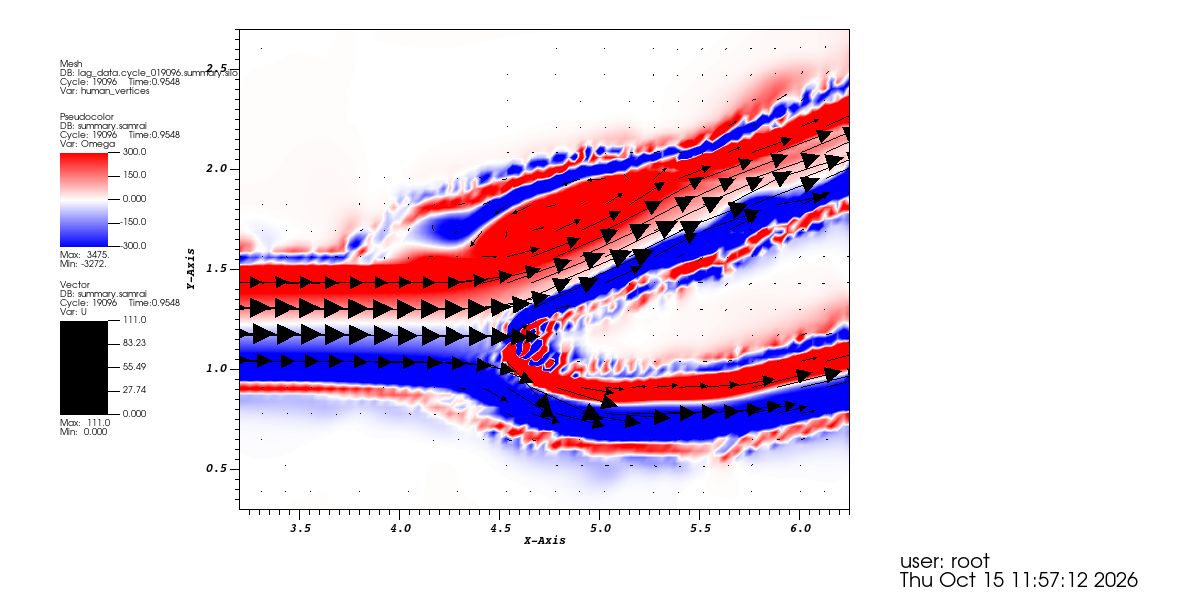
\includegraphics[width=0.48\textwidth]{ch26-5-zoom.png}\hfill
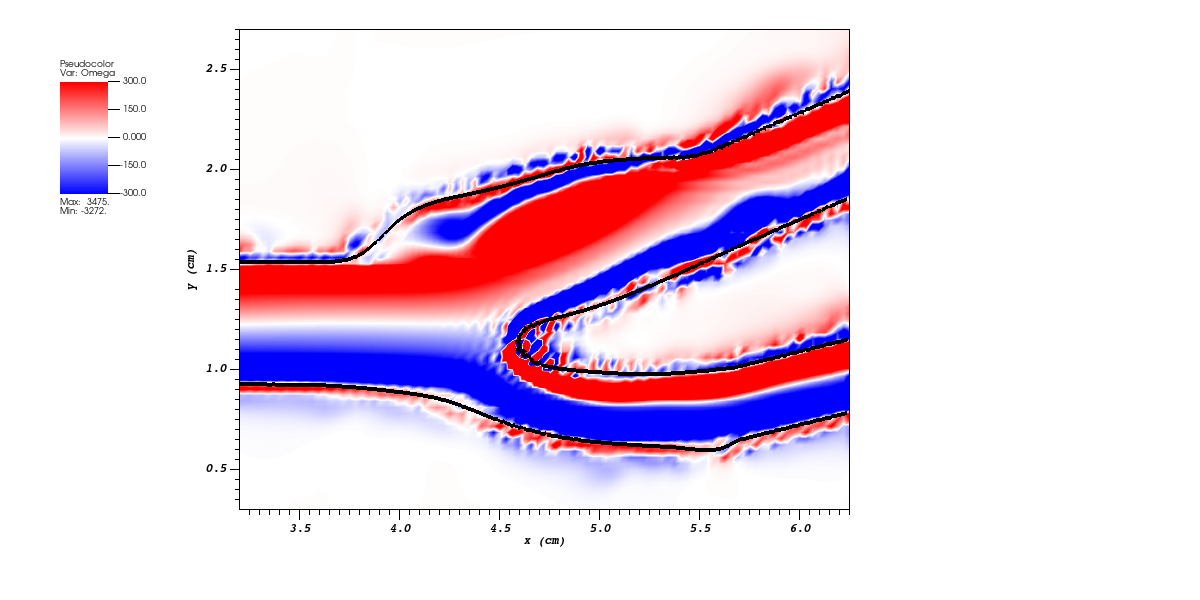
\includegraphics[width=0.48\textwidth]{ch26-8-mesh-edges.png}\\[1mm]
\scriptsize\raggedright Left: the boundary as the Mesh plot of \code{human\_vertices}, one pixel per point, as first drawn: a dotted line that disappears under the vectors. Right: the Mesh plot of \code{human\_mesh}, the spring edges, with \gui{Line width} 3 and \gui{Mesh color} black, the vectors hidden and the annotations cleaned: a continuous wall. A run without springs has no \code{<name>\_mesh}; then \gui{Point size} 6 of the vertices does the job, or the line is thickened afterwards (chapter 30's \code{tools/thicken\_line.py}).
\end{frame}

% 26
\begin{frame}{The polished picture}
\label{fr:final}
\centering
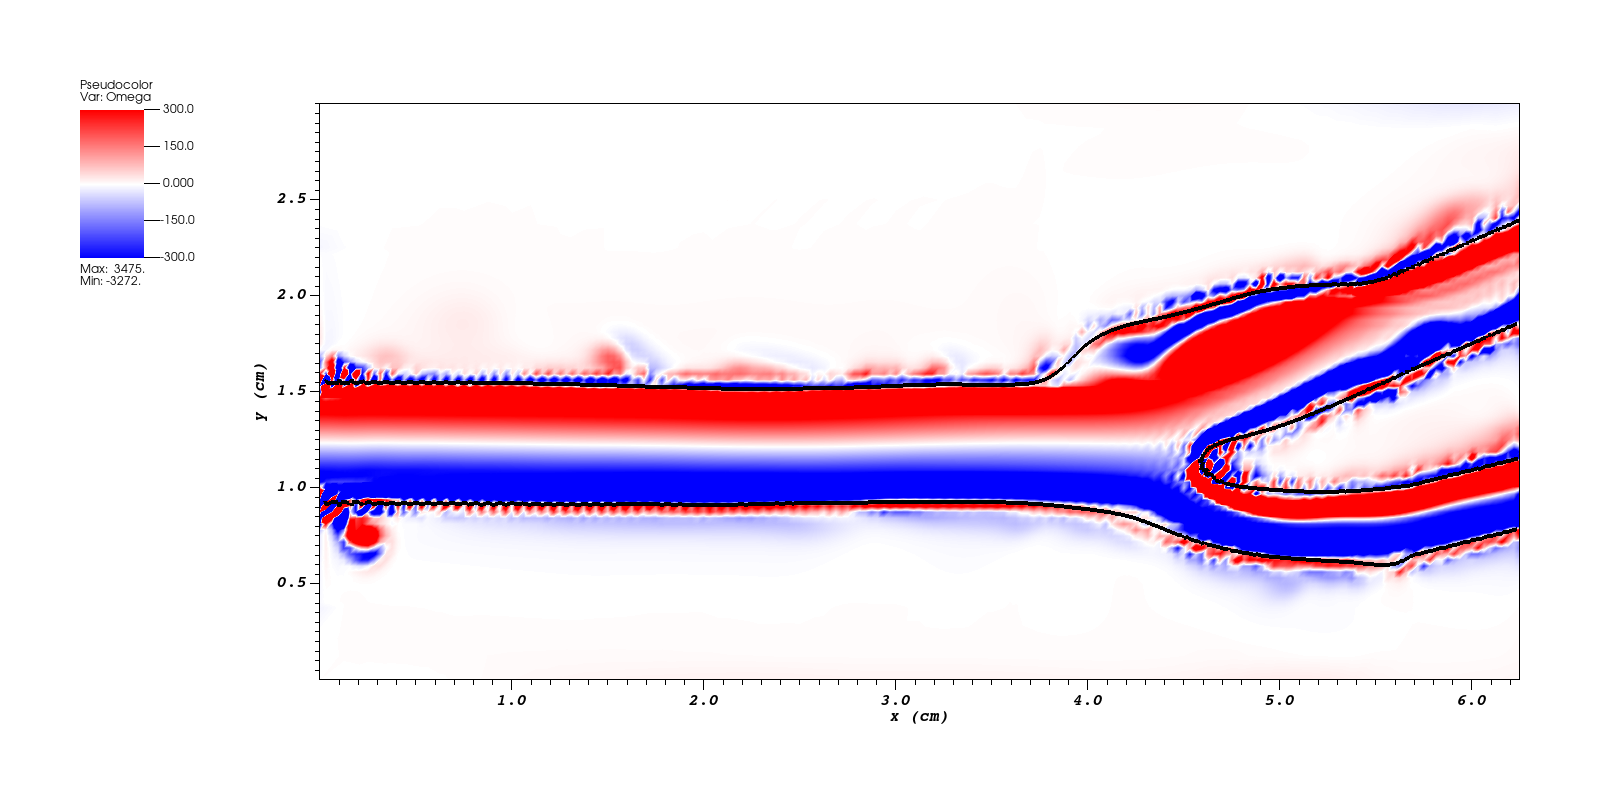
\includegraphics[height=0.72\textheight]{ch26-7-final.png}\\[1mm]
\scriptsize IB/13 human, the systolic peak of the second cycle: vorticity $\pm300$ s$^{-1}$, nodal, \code{difference}; the boundary as the spring mesh in 3-pixel black lines; axes titled in cm; no database name, no user name, no Subset plot, one legend. The same window as slide \ref{fr:points}'s first picture.
\end{frame}

% 27
\begin{frame}{The checklist: making it look better}
\label{fr:checklist}
\footnotesize
\begin{tabular}{@{}L{0.34\textwidth}L{0.6\textwidth}@{}}
\toprule
item & where, and the value this chapter used \\
\midrule
fixed, symmetric limits & Pseudocolor \gui{Data}: about a quarter of the automatic range or less; $\pm300$ \\
nodal centering & Pseudocolor \gui{Data} \gui{Centering}; smooth instead of blocky \\
a diverging table for a signed field & \code{difference}; \code{viridis} for a magnitude \\
opacity under vectors & 70\%; fully opaque otherwise \\
vectors: uniform, fixed number, constant colour, scaled by magnitude & Vector \gui{Sampling}/\gui{Geometry}/\gui{Data}; 3000--5000 at slide size \\
the boundary visible and continuous & Mesh \gui{Line width} 2--4 on \code{<name>\_mesh}, or \gui{Point size} 4--8 px; black \\
the Subset plot VisIt added & deleted \\
no database name, no user name & Annotation \gui{General} \\
axes titled in units, or off & Annotation \gui{2D} \\
one legend, without title and min/max, placed & Annotation \gui{Objects} \\
white background for print & Annotation \gui{Colors} \\
the frame's time, if it matters & a text annotation with \code{\$time} (Annotation \gui{Objects}; chapter 30) \\
saved at a chosen size & \gui{Set save options}; the session saved next to it \\
\bottomrule
\end{tabular}
\end{frame}

% 28
\begin{frame}{The same steps for IB2d}
\label{fr:ib2d}
\begin{columns}[T]
\column{0.52\textwidth}
\scriptsize
\begin{itemize}
  \item IB2d writes \code{viz\_IB2d/} too, as VTK files: \code{lagsPts.*.vtk} (the points), \code{u.*.vtk} (velocity), \code{Omega.*.vtk}, \code{P.*.vtk}, one file per frame per variable, and \code{hier\_IB2d\_data/} for the forces (the 2024 practical, slides 11--27).
  \item \gui{Open} the \emph{group} \code{lagsPts.*.vtk database} (VisIt shows the series as one entry), \gui{Add $\to$ Mesh $\to$ mesh}, \gui{Draw}, point size 8; \gui{Open} \code{u.*.vtk}, \gui{Add $\to$ Vector $\to$ u}; say yes to the \gui{Index} correlation; \gui{Open} \code{Omega.*.vtk}, \gui{Add $\to$ Pseudocolor $\to$ Omega}, then re-add the mesh on top. Each variable is its own database, so the correlation matters more than with IBAMR, and the \gui{Active source} changes with every \gui{Open}.
  \item The attribute values are the IB2d ones: the 2024 deck's vorticity limits were $\pm50$ for the rubber band.
  \item Everything else on these slides is the same: nodal centering, the colour table, annotations, sessions, Save window. Chapter 4b does the IB2d walk-through in full with its own data.
\end{itemize}
\column{0.46\textwidth}
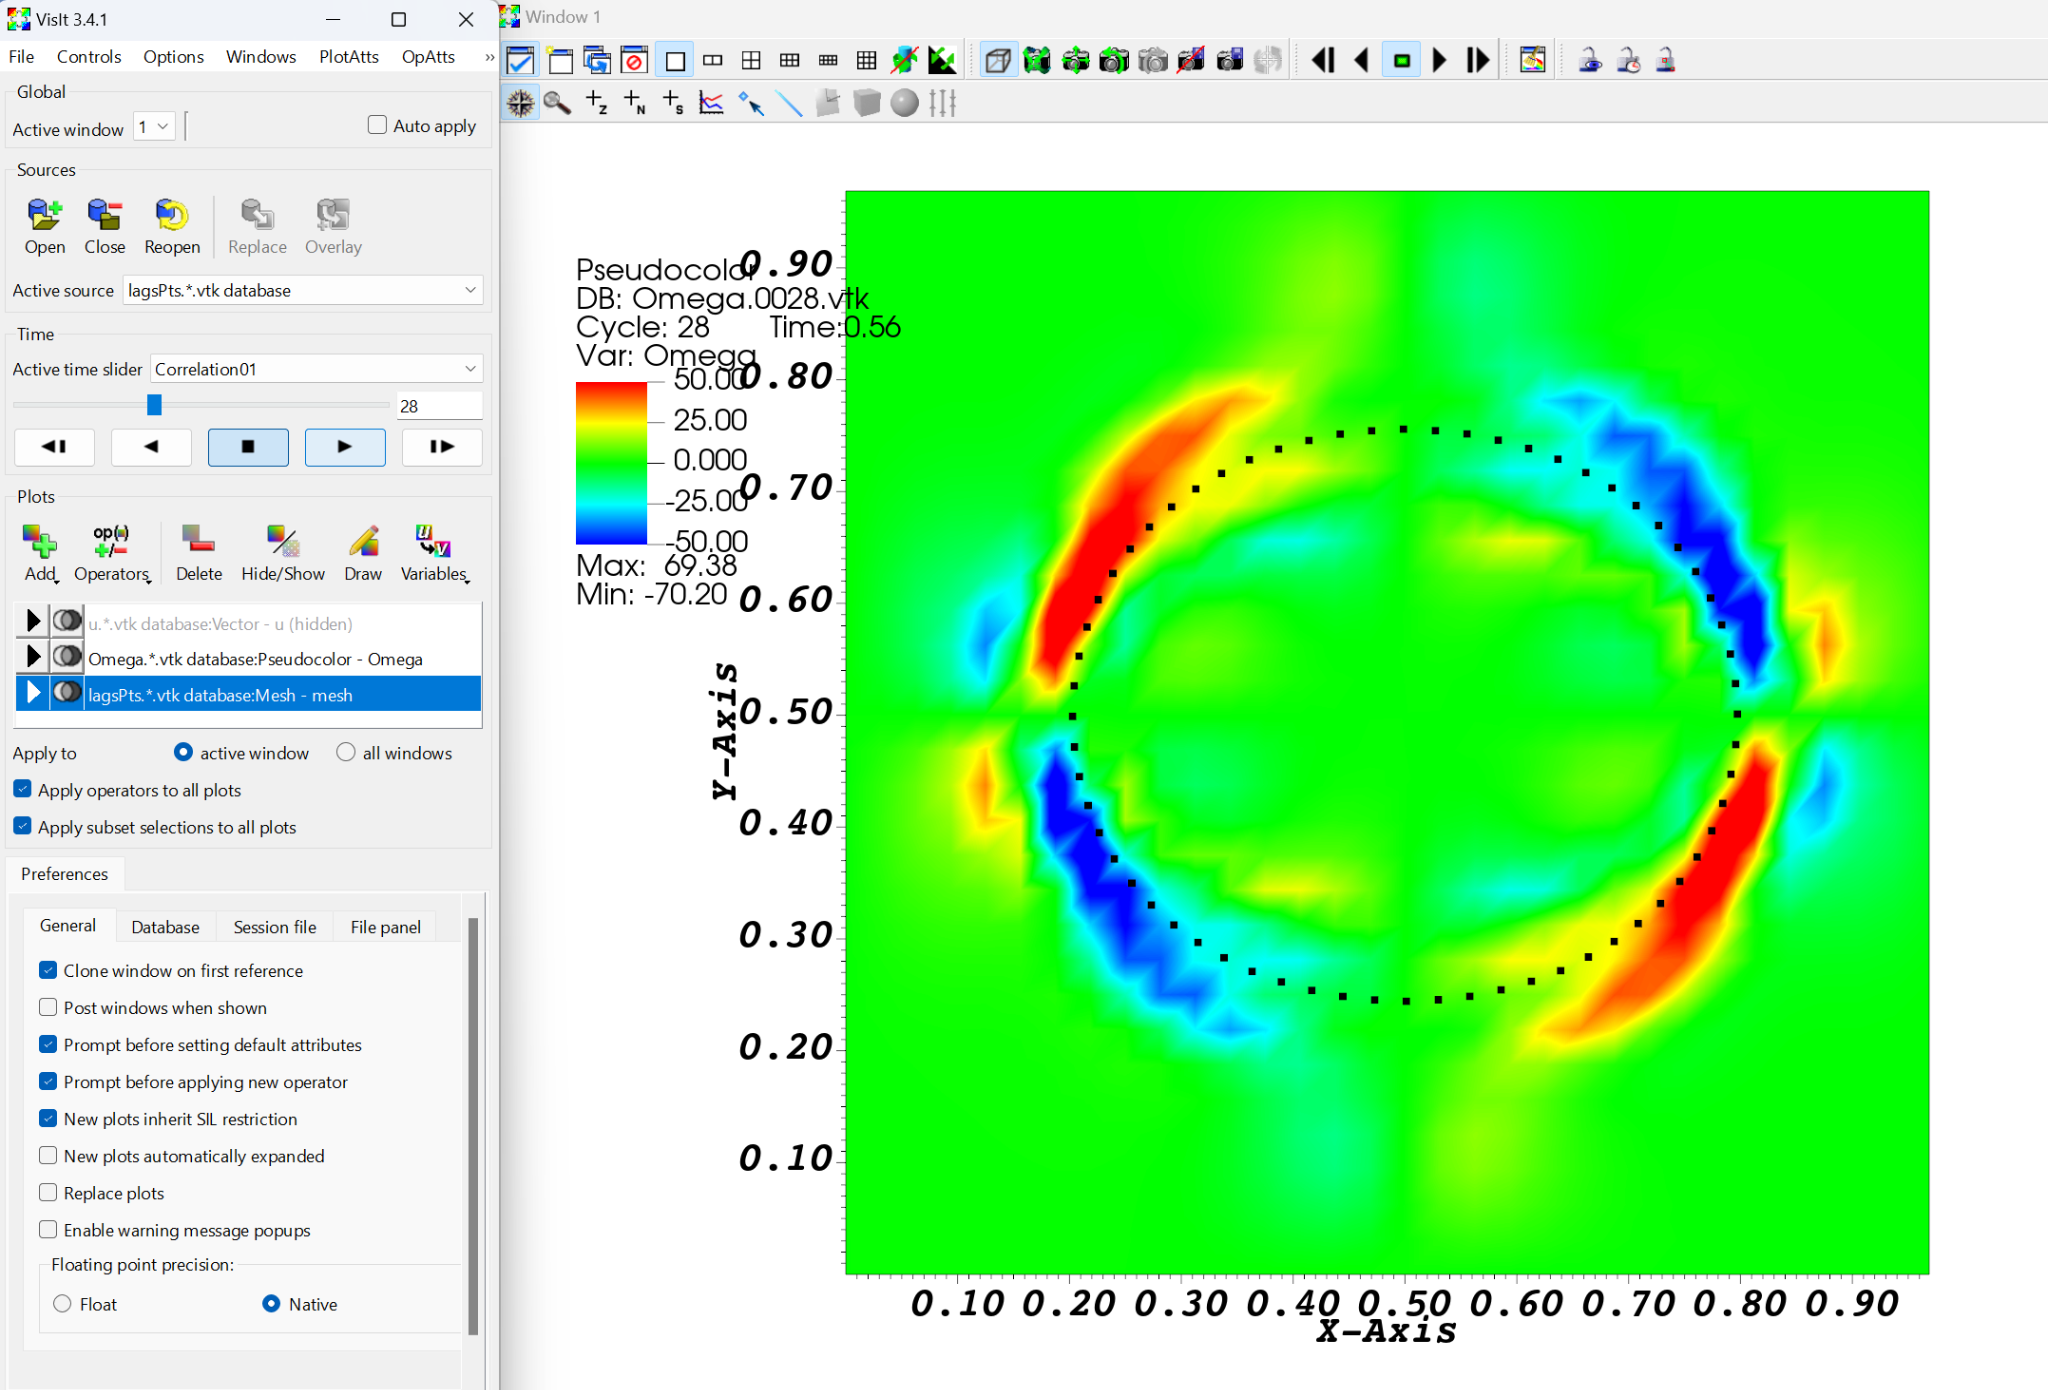
\includegraphics[width=\textwidth]{ch26-gui-tuned-ib2d.png}
\sourcecredit{VisIt 3.4.1 (2024 practical, slide 23): the rubber band at frame 28 with \code{Omega} at $\pm50$, nodal, the mesh re-added on top, the velocity plot hidden; the Correlation01 slider.}
\end{columns}
\end{frame}

% 29
\begin{frame}{The graph supplement (2015): five rules for a figure}
\label{fr:graph}
\footnotesize
\begin{enumerate}
  \item \al{Report in non-dimensional terms where you can:} body lengths per beat, diameters, a Reynolds or Womersley number in the caption; the reader compares across organisms.
  \item \al{Axes that read at the size they will be printed:} titles with units, font sizes set for the final width, no default 10-point labels on a column-width figure.
  \item \al{A colour map that survives greyscale and colourblindness:} \code{viridis} and the diverging \code{difference} do; the rainbow does not. Test by saving once in \code{gray}.
  \item \al{One message per panel:} a colour map, a line plot, or vectors, not all three; hide what you did not come to show.
  \item \al{Reproducible:} the session or the script that made it, saved next to it, so the figure can be remade when the referee asks for a different frame.
\end{enumerate}
\begin{punchbox}
\scriptsize The supplement's examples were three figures on a Drive that is not public; its ``vischeck'' link is dead. The rules stand. Chapter 33 adds the export to MATLAB and Python for the line plots.
\end{punchbox}
\end{frame}

% 30
\begin{frame}{What can go wrong}
\label{fr:wrong}
\scriptsize
\renewcommand{\arraystretch}{0.92}
\begin{tabular}{@{}L{0.36\textwidth}L{0.57\textwidth}@{}}
\toprule
symptom & cause and fix \\
\midrule
nothing appears after \gui{Open} & opening is not drawing: \gui{Add} a plot, then \gui{Draw} \\
the fluid moves, the boundary does not & no database correlation: answer yes at the second \gui{Open}, or \gui{Controls $\to$ Database correlations} \\
``Vector plot yielded no data'' & frame 0 is at rest; move the slider \\
the Pseudocolor hides the points & plots draw in order: add the mesh last, or lower the Pseudocolor's opacity \\
coloured boxes or straight lines you did not ask for & the Subset plot of \code{levels} VisIt adds on opening a SAMRAI database: delete it (hiding keeps its legend) \\
the colours flicker from frame to frame & automatic limits per frame: set \gui{Minimum} and \gui{Maximum} \\
blocky colour map & zonal centering: choose \gui{Nodal} \\
a popup at every frame while saving & \gui{Options $\to$ Preferences}, untick \gui{Enable warning message popups} \\
\code{U\_x} is not in the menu & 0.19 writes the vector \code{U}; use \code{U[0]} as an expression \\
a saved picture is the window's size, not the one asked & \gui{Screen capture} is ticked, or \gui{1:1 aspect ratio} is on in \gui{Set save options} \\
a restored session finds no data & absolute paths inside it: \gui{Restore session with sources} \\
the legend's numbers are unreadable & \gui{Annotation $\to$ Objects}, the legend's font and \gui{Draw min/max} \\
2.x instructions name tabs that do not exist & \gui{Location}, \gui{Form}, \gui{Rendering} became \gui{Sampling}, \gui{Geometry}, \gui{Data} (in 3.0--3.1 \gui{Vectors}, \gui{Glyphs}, \gui{Data}); the controls are the same \\
\bottomrule
\end{tabular}
\end{frame}

% 31
\begin{frame}{What the old decks had that is now Part X}
\label{fr:legacy}
\scriptsize
\begin{tabular}{@{}L{0.46\textwidth}L{0.46\textwidth}@{}}
\toprule
2014--2020 & now \\
\midrule
VisIt 2.5.2 from \code{wci.llnl.gov}; screenshots of a 2014 cluster session on a Mac & VisIt 3.5.0 from \code{visit-dav.github.io}; plot pictures from a run of this series, window screenshots from the 2024 practical (3.4.1) until re-shot \\
sample data on a Google Drive (``flow past a triangle'') & IB/13 or IB/01, made by the reader \\
\code{U\_x}, \code{U\_y} in the variable list & the vector \code{U} and expressions \\
\gui{Location}, \gui{Form}, \gui{Rendering} tabs of the Vector window & \gui{Sampling}, \gui{Geometry}, \gui{Data} \\
Hide/Show the coloured boxes & delete the Subset plot \\
Save movie as MPEG, then ``MPEG is not the best option'': PNG frames + VirtualDub or QuickTime Pro & PNG frames + \code{ffmpeg} (chapter 30), or the CLI \\
``2D or 3D to modify axes'' & the Annotation window's \gui{2D} tab; chapter 27 for 3D \\
12000 vectors (2014) vs 8000 (2020) & 3000--5000 at slide size, uniformly placed \\
the vector scale 0.04 (2014) corrected to 0.4 (2018) & \gui{Scale by magnitude} with \gui{Auto scale} off, set by eye \\
MATLAB export at 600 dpi & VisIt saves raster at any size; curves go to chapter 33 \\
\bottomrule
\end{tabular}
\end{frame}

% 32
\begin{frame}{Exercises}
\label{fr:exercises}
\footnotesize
\begin{enumerate}
  \item Run IB/13 human (or IB/01) and reproduce slide \ref{fr:final}: the same limits, centering, colour table, boundary and annotations. Save the session next to the picture.
  \item Make the same picture of \code{magnitude(U)} with \code{viridis}, then save it with the \code{gray} table: does it still read?
  \item Say no to the correlation at the second \gui{Open}, play, and watch the boundary stay put; then fix it from \gui{Controls $\to$ Database correlations}.
  \item Vectors: 2000, 4000 and 12000 of them on the zoomed bifurcation; which number reads at the width of a column?
  \item Pick the vorticity at the flow divider's apex across the cycle with \gui{Do time curve}; export the curve (chapter 29 does this properly).
  \item Leave the \code{levels} Subset plot in and play: where is the fine level at the start and at the peak? Then untick level 1 in the Subset window.
  \item Restore the session on the horse run with \gui{Restore session with sources}: which attributes need changing for a box three times the size?
\end{enumerate}
\end{frame}

% 33
\begin{frame}{Rules of thumb}
\label{fr:thumb}
\small
\begin{itemize}
  \item Open the \code{.visit} file, not a frame; open both files; say yes to the correlation.
  \item Opening is not drawing. Add, then Draw. Delete the plot you did not add.
  \item Fix the limits, go nodal, pick the table for the sign of the field.
  \item Vectors: uniform, a few thousand, one colour, scaled by magnitude.
  \item Draw the boundary as the spring mesh with a line width, or as points large enough to join.
  \item Turn off the database and user names before anyone else sees the picture.
  \item Save the session next to the figure.
\end{itemize}
\end{frame}

% 34
\begin{frame}{Summary}
\label{fr:summary}
\footnotesize
\begin{enumerate}
  \item An IBAMR run gives VisIt two time series: the fluid in \code{dumps.visit} and the points in \code{lag\_data.visit}; opened as two correlated sources they move together under one slider.
  \item The boundary is a Mesh plot of \code{<name>\_mesh} (the springs, with a line width) or \code{<name>\_vertices}; the fields are Pseudocolor and Vector plots of \code{Omega}, \code{P}, \code{U} and expressions of them; the Subset plot of \code{levels} that VisIt adds on open is deleted.
  \item Five attribute settings make the difference between a first picture and a figure: fixed symmetric limits, nodal centering, a colour table that fits the field, uniformly placed vectors in one colour, a visible boundary.
  \item The Annotation window removes what the figure does not need and adds what it does; Set save options sets the size; the session records it all.
  \item IB2d's \code{.vtk} output takes the same route, one database per variable.
\end{enumerate}
\begin{homebox}
\footnotesize Next: chapter 28, the Lagrangian and finite-element data (the Silo points and the ExodusII meshes with their displacements), then chapter 33, the data formats and the way out to Python and MATLAB.
\end{homebox}
\end{frame}

% 35
\begin{frame}{Recordings and screenshots}
\label{fr:videos}
\small The 2020 Zoom recording of \emph{VISIT -- How to plot IBAMR Data} (Lecture 1 of the 2020 visualization series) and the 2024 recording of the IB2d practical are listed in the front matter's video list (chapter 0.1) and not incorporated. The window screenshots of those two decks are reused here as they were (VisIt 2.5.2 and 3.4.1, credited on each slide); the plan to re-shoot them in 3.5.0 on the IB/13 run, with the file names and what each must show, is \code{plan/visit-screenshots-todo.md}.
\end{frame}

% 36
\begin{frame}{References and credits}
\label{fr:refs}
\scriptsize
\begin{itemize}
  \item VisIt 3.5.0, Lawrence Livermore National Laboratory: \url{https://visit-dav.github.io/visit-website/}; the VisIt User Manual (\url{https://visit-sphinx-github-user-manual.readthedocs.io/}) for every window named here; the Python CLI manual for chapter 32.
  \item H. Childs et al., \emph{VisIt: an end-user tool for visualizing and analyzing very large data}, in High Performance Visualization (2012) 357--372.
  \item The course material: \emph{VISIT -- How to plot IBAMR Data} (2020); \emph{IB2D Practical} (2024); \emph{VISIT -- How to make it look better} (2013, ed.\ 2019); the 2015 course lectures 10 and 4A (graph supplement); the 2011--2017 session files.
  \item The data: example IB/13 (human case) of this series, IBAMR 0.19.0, four cores; the plot pictures by \code{wsl/final/visit\_ch26\_renders.sh} (VisIt 3.5.0, headless); the window screenshots from the 2020 and 2024 decks as credited.
\end{itemize}
\end{frame}

\end{document}
